\documentclass[11pt,oneside,chapters]{starlink}

\usepackage{amsfonts}
\usepackage{longtable}
\usepackage{amsmath}
\usepackage{siunitx}

\stardoccategory {Starlink Cookbook}
\stardocinitials {SC}
\stardoccopyright{Copyright \copyright\ 2021 East Asian Observatory}
\stardocnumber   {22}
\stardoctitle    {The POL-2 Data Reduction Cookbook}
\stardocversion  {1.1}
\stardocabstract {
  This cookbook provides an introduction to POL-2 data reduction,
  using the Starlink facilities \smurf (the Sub-Millimetre
  User Reduction Facility) and in particular its command
  \poltwomap. This cookbook illustrates the various steps
  required to reduce the data, including an overview of the method. It
  also describes how to calibrate and display the data as images or
  vector maps.}

\stardocauthors{H.\ A.\ L.\ Parsons, D.\ S.\ Berry,
  M.\ G.\ Rawlings, and S.\ F.\ Graves}

\stardocdate{2021 July 15}

%-------------------------------------------------------------------

% Local Definitions
\newcommand{\xparam}[2]{\xref{#2}{sun258}{#1}}
\providecommand{\PGPLOTref}{\htmladdnormallink{PGPLOT}{http://www.astro.caltech.edu/~tjp/pgplot/}}

%-------------------------------------------------------------------



\begin{document}
\scfrontmatter





% Acronyms section
\Acronyms

\begin{table}[h!]
\begin{tabular}{ll}
\textbf{CADC}   & Canadian Astronomy Data Centre\\
\textbf{FCF}    & Flux Conversion Factor\\
\textbf{FITS}   & Flexible Image Transport System\\
\textbf{GAIA}   & Graphical Astronomy and Image Analysis tool\\
\textbf{HWP}    & Half-Wave Plate\\
\textbf{ITC}    & Integration Time Calculator\\
\textbf{I}      & Total intensity \\
\textbf{IP}     & Instrumental Polarisation \\
\textbf{JCMT}   & James Clerk Maxwell Telescope\\
\textbf{NDF}    & Extensible N-Dimensional Data Format\\
\textbf{P}      & Percentage polarisation \\
\textbf{PCA}    & Principal Component Analysis \\
\textbf{I$_{p}$}     & Polarised intensity \\
\textbf{SCUBA-2}& Submillimetre Common User Bolometer Array-2\\
\textbf{SMURF}  & Sub-Millimetre User Reduction Facility\\
\textbf{SNR}    & Signal-to-noise ratio\\
\textbf{SUN}    & Starlink User Note\\
\textbf{WCS}    & World Coordinate System\\
\end{tabular}
\end{table}


\newpage
\chapter{Introduction}
\label{sec:intro}

% set up page numbers in arabic numerals and restart from 1
\renewcommand{\thepage}{\arabic{page}}
\setcounter{page}{1}

\section{This cookbook}

This guide is designed to instruct POL-2 users on the best ways to
reduce and visualise their data using \starlink\ packages:
\smurf \cite{smurf}, \Kappa \cite{kappa}, \polpack \cite{polpack}
and \gaia \cite{gaia}.

This guide covers the following topics.
\begin{itemize}
\itemsep0em
\item \cref{Chapter}{sec:intro}{Chapter 1} -- Computer resources you'll need before getting started.
\item \cref{Chapter}{sec:pol2}{Chapter 2} -- A description of POL-2 and its observing modes.
\item \cref{Chapter}{sec:dr}{Chapter 3} -- POL-2 Data Reduction - The Theory
\item \cref{Chapter}{sec:rundr}{Chapter 4} -- POL-2 Data Reduction - Running pol2map
\item \cref{Chapter}{sec:display}{Chapter 5} -- POL-2 Image Display
\item \cref{Chapter}{sec:advanced}{Chapter 6} -- POL-2 Advanced Data Reduction

\end{itemize}

Throughout this document, a percent sign (\texttt{\%}) is used to
represent the Unix shell prompt. What follows each \texttt{\%} will be
the text that should be typed by the user to initiate the described action.

\section{\xlabel{computing} Before you start: computing resources}
\label{sec:computing}

Compared to SCUBA-2 observations, POL-2 observations are far less memory intensive to reduce.
POL-2 time-series data is down-sampled to 2Hz within the reduction process. Assuming a typical 35
minute POL-2 observation, the reduction requires 35 GB of memory (in comparison to SCUBA-2
maps that may require up to 96 GB of memory).

The main consideration for POL-2 reductions is processing power. PCA calculations in
makemap can be lengthy so fast processors with lots of cores are advised.


\section{\xlabel{software}Before you start: software}

This manual uses software from \starlink\ packages: \smurf\
\cite{smurf}, \Kappa\ \cite{kappa}, \polpack \cite{polpack} and \gaia\ \cite{gaia}.
Starlink software must be installed on your system, and Starlink
aliases and environment variables must be defined before attempting
to reduce any SCUBA-2 data (see section \ref{sec:starinit}).

\subsection{Data formats}
\label{sec:ndf}

Data files for POL-2 are the same as for SCUBA-2 and use
the Starlink N-dimensional Data Format (NDF,
see Jenness et al.\ 2014\cite{ndf}), a hierarchical format which allows
additional data and metadata to be stored within a single file. \Kappa\
contains \xref{many commands}{sun95} {ap_classified}\ for examining and
manipulating NDF structures. The introductory sections of the \Kappa\
document (\xref{SUN/95}{sun95}{}) contain much useful information on
the contents of an NDF structure and how to manipulate them.

A single NDF structure describes a single data array with associated
meta-data. NDFs are usually stored within files of type ``\verb+.sdf+''.
In most cases (but not all), a single \verb+.sdf+ file will contain just
one top-level NDF structure, and the NDF can be referred to simply by
giving the name of the file (with or without the ``\verb+.sdf+'' prefix).
In many cases, a top-level NDF containing JCMT data will contain other
``extension'' NDFs buried inside them at a lower level. For instance, raw
files contain a number of NDF components which store observation-specific
data necessary for subsequent processing. The contents of these (and
other NDF) files may be listed with \HDSTRACEref. Each file holding raw
JCMT data on disk is also known as a `sub-scan'.

The main components of any NDF structure are:
\begin{itemize}
\item An array of numerical data (may have up to seven
dimensions---usually three for JCMT data);
\item An array of variance values corresponding to the numerical data
values;
\item An array holding up to eight boolean flags (known as ``quality
flags'') for each pixel;
\item World Coordinate System information;
\item History;
\item Data units
\item Other extensions items. These are defined by particular packages,
but usually include a list of FITS-like headers together with provenance
information that indicates how the NDF was created. Raw JCMT files also
include extensions that define the state of the telescope and instrument
at each time slice within the observation.
\end{itemize}

The \convert\ package contains commands \xref{\task{fits2ndf}}{sun55}{FITS2NDF} and
\xref{\task{ndf2fits}}{sun55}{NDF2FITS} that allow interchange between FITS
and NDF format.

\subsection{Initialising Starlink}
\label{sec:starinit}

The commands and environment variables needed to start up the required
Starlink packages (\smurf \cite{smurf}, \Kappa, \emph{etc.}) must first
be defined. For C shells (csh, tcsh), do:

\begin{terminalv}
% setenv STARLINK_DIR <path to the starlink installation>
% source $STARLINK_DIR/etc/login
% source $STARLINK_DIR/etc/cshrc
\end{terminalv}

before using any Starlink commands. For Bourne shells (sh, bash, zsh), do:

\begin{terminalv}
% export STARLINK_DIR=<path to the starlink installation>
% source $STARLINK_DIR/etc/profile
\end{terminalv}

\subsection{KAPPA and SMURF for data processing}
\label{sec:packinit}

The Sub-Millimetre User Reduction Facility, or \textsc{Smurf},
contains the Dynamic Iterative Map-Maker, which will process
SCUBA-2 time-series data into images (see \smurfsun). \textsc{Kappa} meanwhile is
an application package comprising general-purpose commands mostly for
manipulating and visualising NDF data (see \kappasun). Before starting
any data reduction you will want to initiate both \textsc{Smurf} and
\textsc{Kappa}.

\begin{terminalv}
% smurf
% kappa
\end{terminalv}

After entering the above commands, you can access the help information
for either package by typing \texttt{smurfhelp} or
\texttt{kaphelp} respectively in a terminal, or by using the
\task{showme} facility to access the hypertext documentation. See
\cref{Section}{sec:help}{How to get help} for more information.



\begin{tip}
The .sdf extension on filenames need not be specified when running most
Starlink commands (the exception is \picard).
\end{tip}


\subsection{GAIA for viewing your images and vector maps}
Images and vector maps can be displayed and analysed using \gaia\ (see
\gaiasun) - an interactive GUI-driven tool that incorporates facilities
such as vector selection, vector binning, source detection, photometry
and the ability to query and overlay on-line or local catalogues.
\begin{terminalv}
% gaia map.sdf
\end{terminalv}

Alternatively, the \Kappa\ package includes many visualisation commands
that can be run from the shell comand-line or incorporated easily into your
own scripts---see Appendix ``\xref{Classified KAPPA commands}{sun95}{cl_datadisplay}''
in SUN/95. These tools are particularly useful for creating more complex
composite plots including multiple images, line-plots, \emph{etc}, such
as the multi-image plots in \cref{Section}{sec:itermaps}{Monitoring the
map at the end of each iteration}.


\subsection{\xlabel{help}How to get help}
\label{sec:help}

\begin{table}[h!]
\begin{tabular}{p{2.3cm}|p{7.3cm}|p{5cm}}
\hline
\textbf{Help\newline command} & \textbf{Description} & \textbf{Usage}\\
\hline
\task{showme} & If you know the name of the Starlink document you want to view,
                use \task{showme}. When run, it launches a new webpage or tab
                displaying the hypertext version of the document. &
\texttt{\%~showme~sun95}\\
\hline
\task{findme} & \task{findme} searches Starlink documents for a keyword. When
                run, it launches a new webpage or tab listing the results. &
                \texttt{\% findme~kappa}\\
\hline
\task{docfind} & \task{docfind} searches the internal list files for keywords. It then
                 searches the document titles. The result is displayed using the
                 Unix \task{more} command. & \texttt{\%~docfind~kappa}\\
\hline
Run routines with prompts & You can run any routine with the option
                            \texttt{prompt} after the command. This will
                            prompt for every parameter available. If you
                            then want a further description of any parameter
                            type  \texttt{?} at the relevant prompt. &
                            \texttt{\%~makemap~prompt~\newline\~\%~REF~-~Ref.~NDF~/!/$>$~?}\\
\hline
Google & A simple Google search such as ``\texttt{starlink kappa fitslist}''
will usually return links to the appropriatre documents. However, be
aware that the results may include links to out of date versions of the
document hosted at non-Starlink sites. Always look for results in
\texttt{"www.starlink.ac.uk/docs} (or \texttt{"www.starlink.ac.uk/devdocs}
for the cutting-edge development version of the document). & \\
\hline
\end{tabular}
\end{table}


\newpage
\chapter{\xlabel{pol2_overview}POL-2 Overview}
\label{sec:pol2}
\section{\xlabel{pol2}The instrument}

The POL-2 instrument is a linear polarimetry module for the
Submillimetre Common User Bolometer Array-2 (SCUBA-2), a 10,000
bolometer camera on the JCMT \cite{Friberg} \cite{Bastien2011}.  POL-2
in itself is not a detector - thus requiring SCUBA-2 and its detectors
for operation. SCUBA-2 operates simultaneously at both 850 and
\SI{450}{\micro\metre}. The POL-2 instrument is currently commissioned
at \SI{850}{\micro\metre} only.

\begin{figure}[t!]
\begin{center}
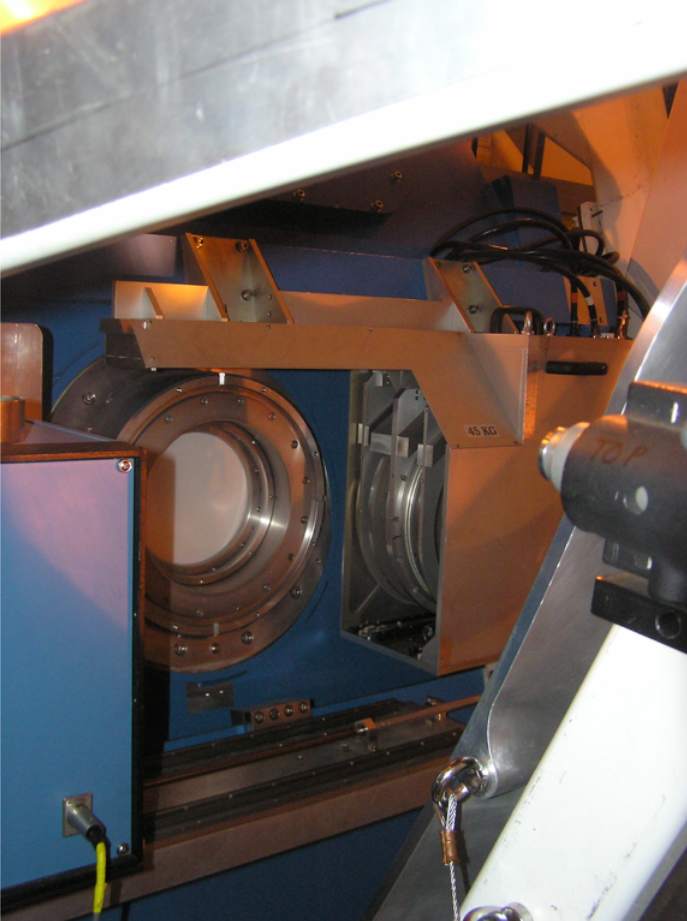
\includegraphics[width=0.45\linewidth]{pol2-out-of-beam.png}
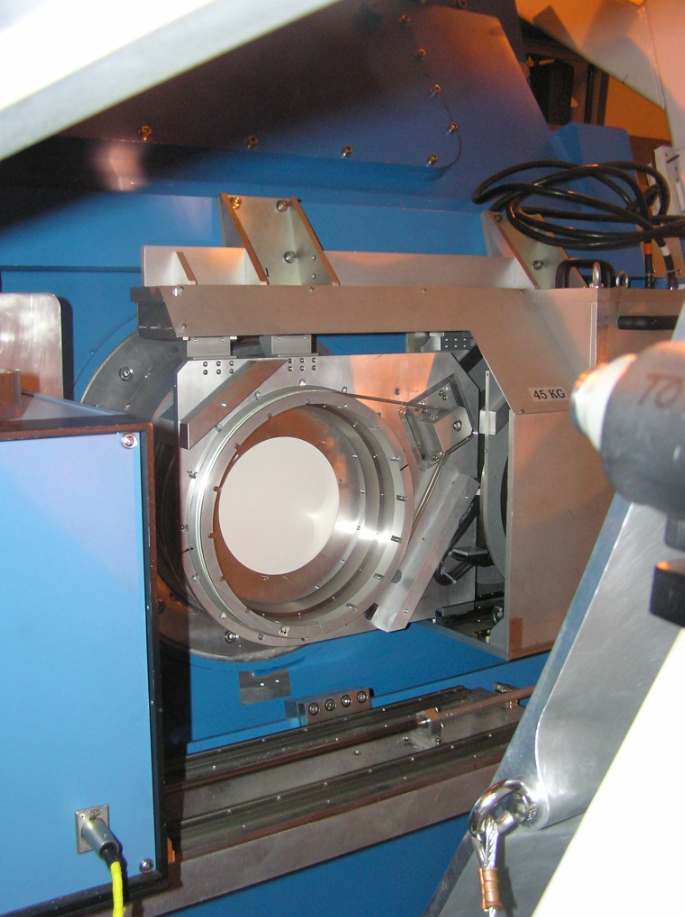
\includegraphics[width=0.45\linewidth]{pol2-in-beam.png}
\label{fig:pol2sc2}
\caption [POL-2 mounted on SCUBA-2]{POL-2 mounted on the front of
  SCUBA-2.  The left image shows the SCUBA-2 window. The right image
  shows the components of POL-2 inserted in front of the SCUBA-2
  window: the calibrator grid, rotating half-wave-plate (HWP) and the
  analyser grid. The calibrator grid is only inserted for test
  purposes.}
\end{center}
\end{figure}

\subsection*{Polarisation}

In polarimetric terms light is conventionally described by the four
Stokes parameters: $I$, $Q$, $U$ and $V$.


$I$ is the total intensity; $Q$ is the radiation linearly polarised in
the direction parallel or perpendicular to the reference plane. $U$ is
the radiation linearly polarised in the directions 45$^{\circ }$ to
the reference plane; and $V$ is the circularly polarised radiation.

POL-2 is designed to characterise linear polarisation.  The $V$
parameter, consequently, is not discussed further with the focus on $I$,
$Q$ and $U$.

The linear Polarised Intensity (I$_{p}$) and  polarisation angle
($\theta$) can be described as:

\begin{equation}
I_{p} = \sqrt{Q^{2}+U^{2}}
\end{equation}
\begin{equation}
\theta = 0.5\arctan(U/Q)
\end{equation}

with Q and U related to the polarisation angle and the polarised intensity by:

\begin{equation}
Q = I_{p} \text{cos}(2\theta)
\end{equation}
\begin{equation}
U = I_{p} \text{sin}(2\theta)
\end{equation}

where

\begin{equation}
Q = Q_{m} - I . IP_{q}
\end{equation}
\begin{equation}
U = U_{m} - I . IP_{u}
\end{equation}

where Q$_{m}$ and U$_{m}$ are the measured values of Q and U.  I is
the astronomical total intensity.  IP is the instrumental
polarisation. The IP affects both Q (\emph{via} IP$_{q}$) and U
(\emph{via} IP$_{u}$).


\subsection*{How POL-2 works}

POL-2 is located in front of the window to the SCUBA-2 instrument (as
is seen in Figure~\ref{fig:pol2sc2}), and covers the full field of
view of SCUBA-2. The POL-2 polarimeter uses three optical components
that cover the full field of SCUBA-2:

\begin{enumerate}
\item a wire-grid polariser used as a calibrator (only included in the
  beam for test purposes)
\item a Half-Wave Plate (HWP)
\item a second wire-grid polariser used as an analyser
\end{enumerate}

These components can be seen in Figure~\ref{fig:pol2sc2}.  A schematic
of POL-2 is given in Figure~\ref{fig:pol2sc2diagram}.

\begin{figure}[t!]
\begin{center}
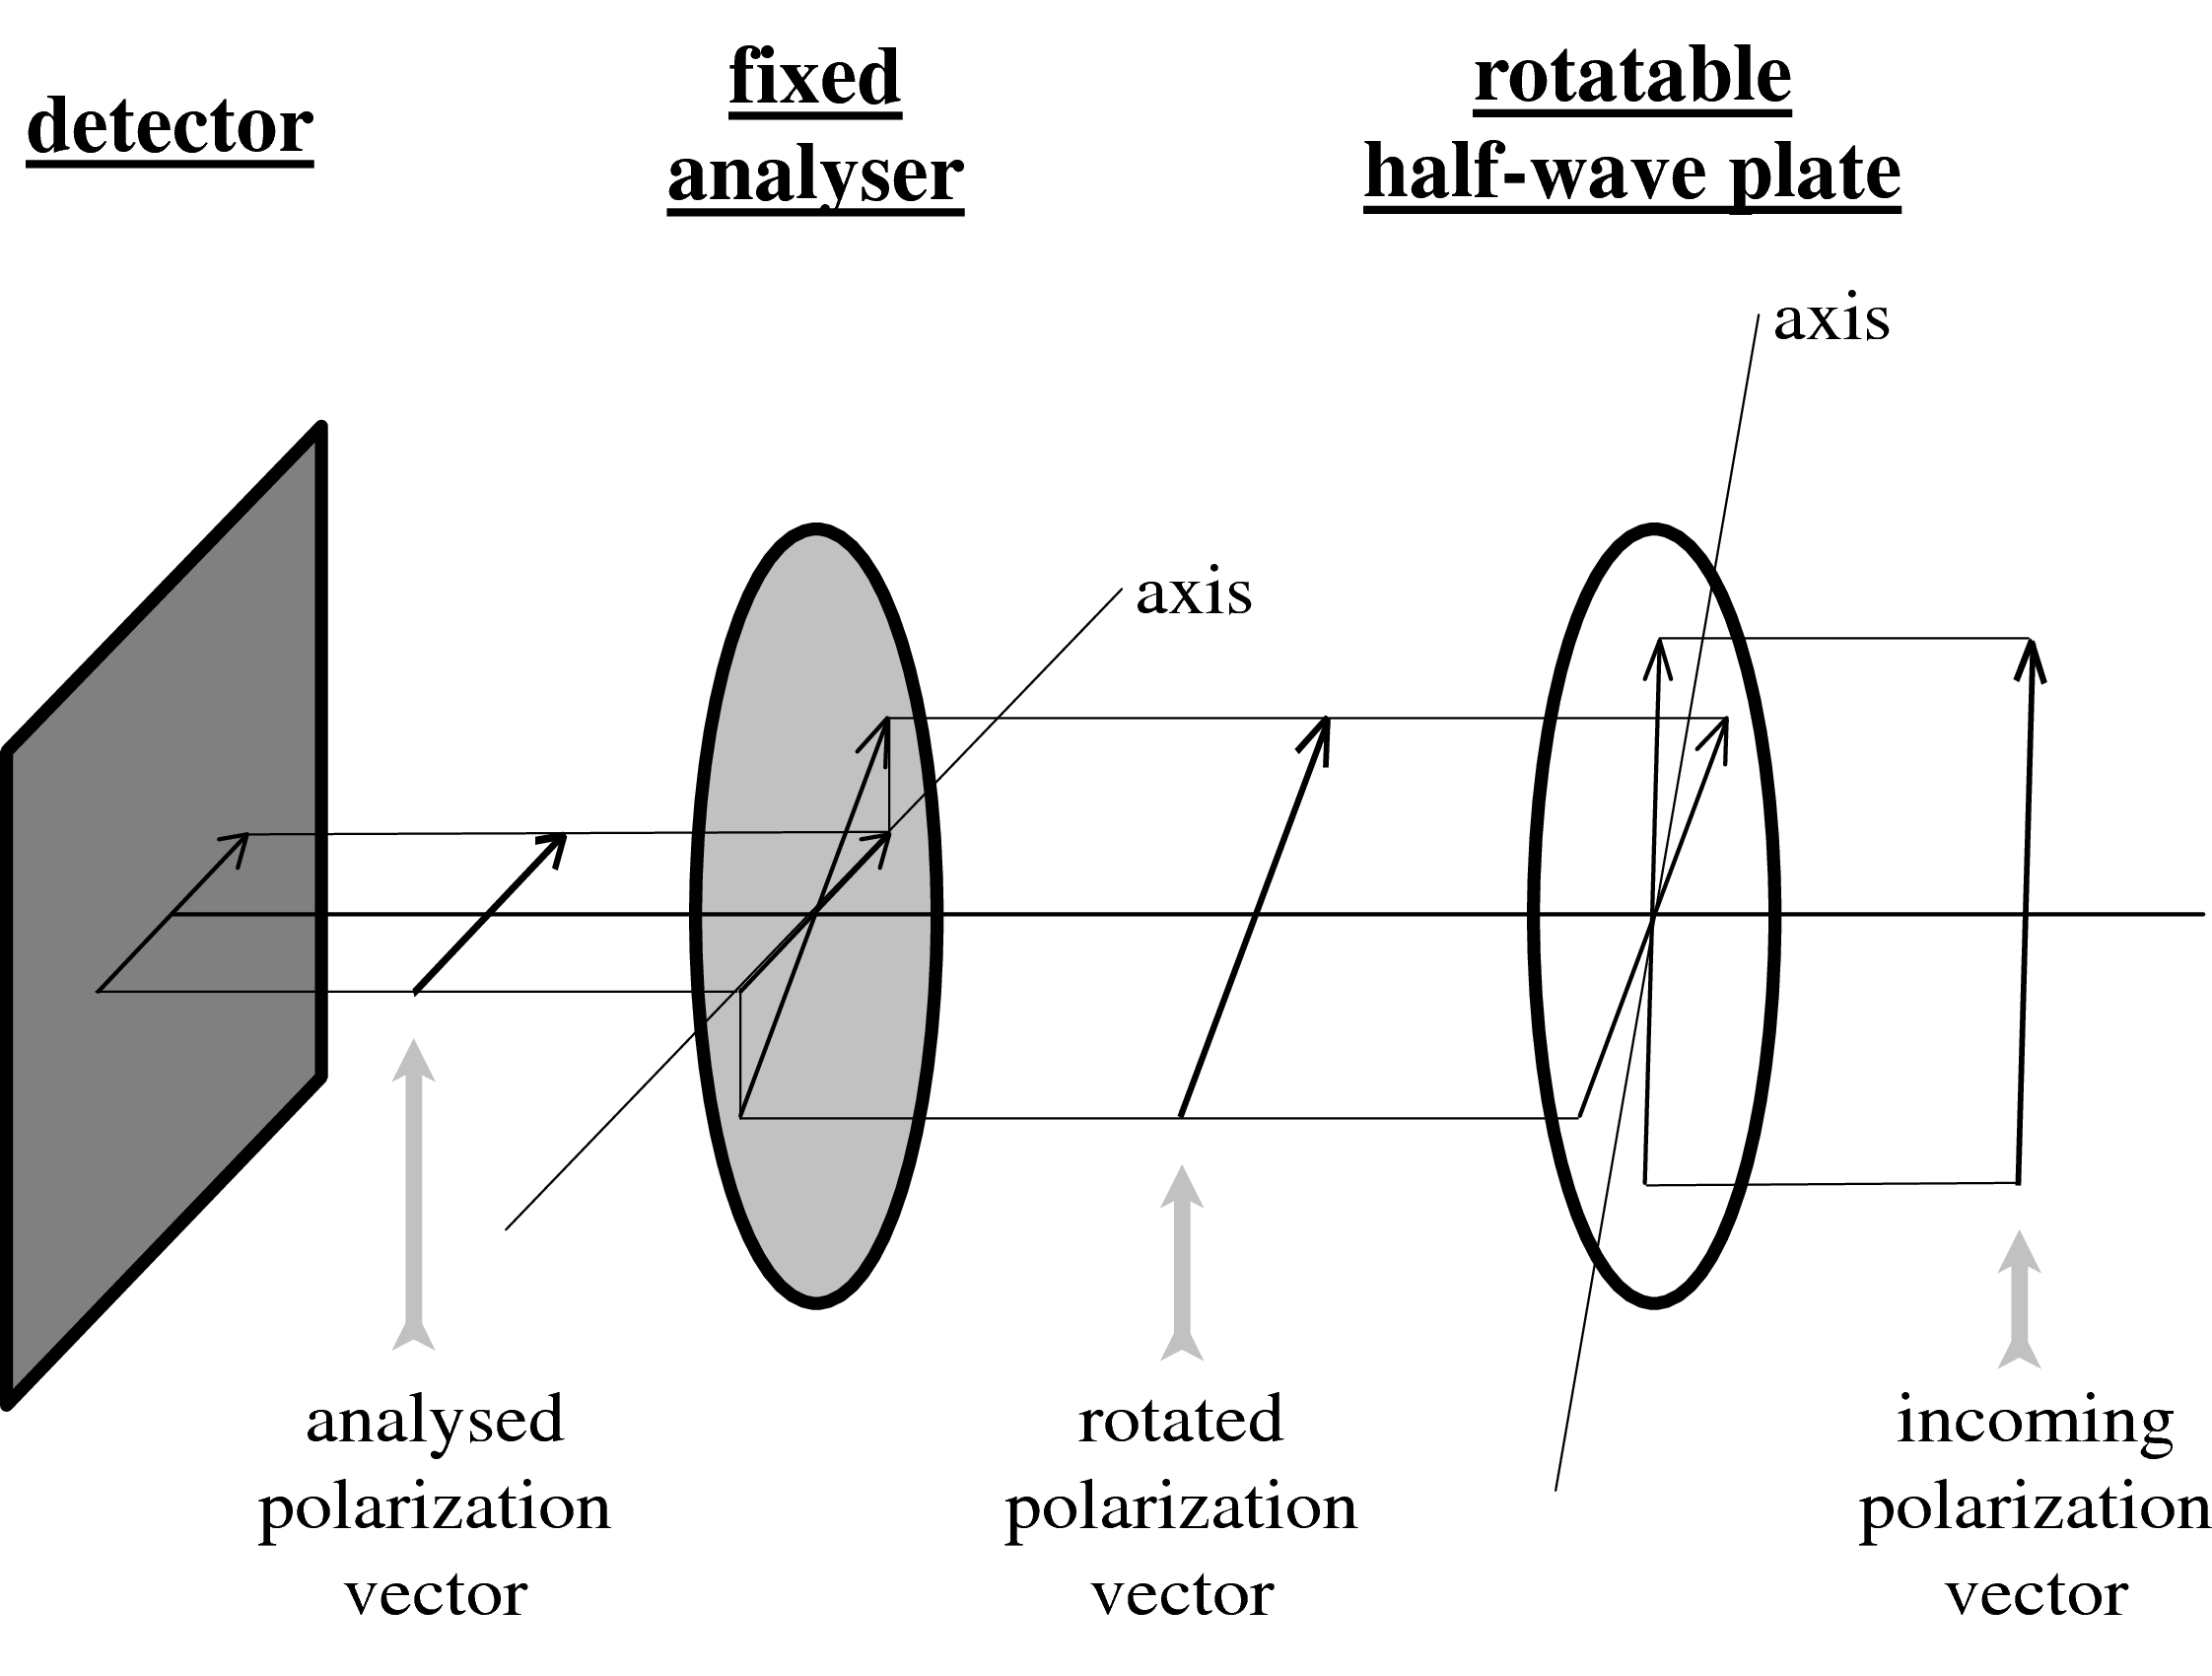
\includegraphics[width=0.8\linewidth]{singopt.png}
\caption [POL-2 optical components]{ The main optical components in a
  typical single-beam imaging polarimeter such as POL-2 (taken from
  SUN/223).}
\label{fig:pol2sc2diagram}
\end{center}
\end{figure}

Rotating the HWP rotates any linearly polarised component of incoming
radiation. The HWP rotates this incoming linear polarisation with
twice the speed of the HWP angle ($\delta$) producing the
\emph{effective analyser} position ($\phi$ - as defined in
\xref{the POLPACK documentation}{sun223} {thepolarimeter}), such that:


\begin{equation}
\phi = 2 \delta
\end{equation}


The rotating linearly polarised component is transmitted or reflected
by the grid, causing a modulation in the transmitted intensity.
The amplitude of the polarised component transmitted by the polariser is
$\sim$cos($\phi$) while the power is $\sim$cos$^{2}$($\phi$).

\begin{figure}[t!]
\begin{center}
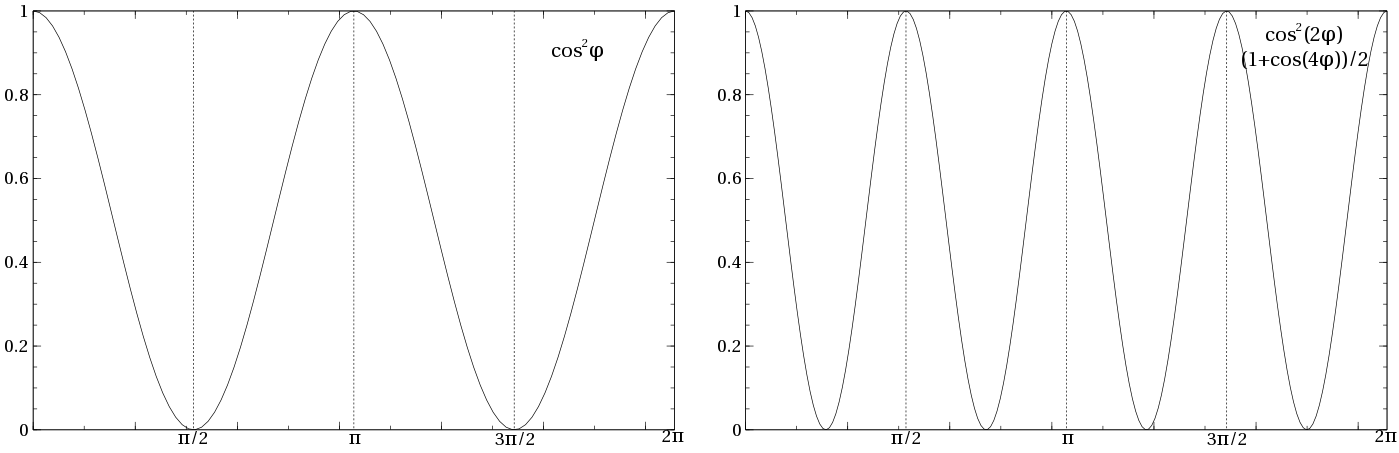
\includegraphics[width=0.95\linewidth]{hwp-modulation-basic.png}
\label{fig:hwp-modulation-basic}
\caption [Modulation by the HWP - basic description]{ Left: If there
  was a single rotating analyser this would be the resulting curve of
  the power transmitted of the linearly polarised component.
  Right: With the HWP the linearly polarised component is
  rotated at twice the speed. It may be useful to remind the reader of
  the trigonometric identity: \\ cos$^{2}$x = 0.5(1+cos(2x))}
\end{center}
\end{figure}


The radiation passing through the polarimeter is detected by
SCUBA-2. The detected intensity (I$_{detected}$) is a combination of
\emph{both} the unpolarised intensity (I$_{unpolarised}$) and the
linearly polarised intensity (I$_{p}$)\footnote{The total intensity of
the source, $I$, is $I_{unpolarised} + I_{p}$.}. This detected intensity can be
described by:

\begin{equation}
I_{detected} = \frac{I_{unpolarised}}{2}+ I_{p}\cdot\left(\frac{1+\cos(2\phi - 2\theta)}{2} \right)
\end{equation}

with the above equation being in terms of the effective analyser
angle, $\phi$ and the angle of the polarisation ($\theta)$.
This can also be expressed in terms of the  the HWP angle ($\delta$).

\begin{equation}
\label{eqn:idet}
I_{detected} = \frac{I_{unpolarised}}{2}+I_{p}\cdot\left(\frac{1+\cos(4\delta - 2\theta)}{2} \right)
\end{equation}




\subsection*{The Half-Wave Plate}

As described in the POL-2 commissioning document the HWP is
constructed from five individual synthetic sapphire layers
approximately 0.9 mm thick and 200 mm in diameter. The transmission
properties of sapphire are generally good at the SCUBA-2 wavelengths
but are dependent on the thickness and ambient temperature. The total
effective transmission of the HWP integrated across the 850 and
\SI{450}{\micro\metre} filter bands are about 86\% and 57\%
respectively (Savini et al. 2009 - insert full reference).

The HWP rotates the incoming linear polarisation with twice the speed
of the wave plate angle.  The HWP is typically rotated at 2Hz,
providing a fast modulation of any linear polarisation by 8Hz (see
equation~\ref{eqn:idet}).  The data acquisition rate is ~175Hz, yielding
20 samples per cycle.  The atmosphere is stable on the order of 2Hz and
can be removed.


\begin{figure}[t!]
\begin{center}
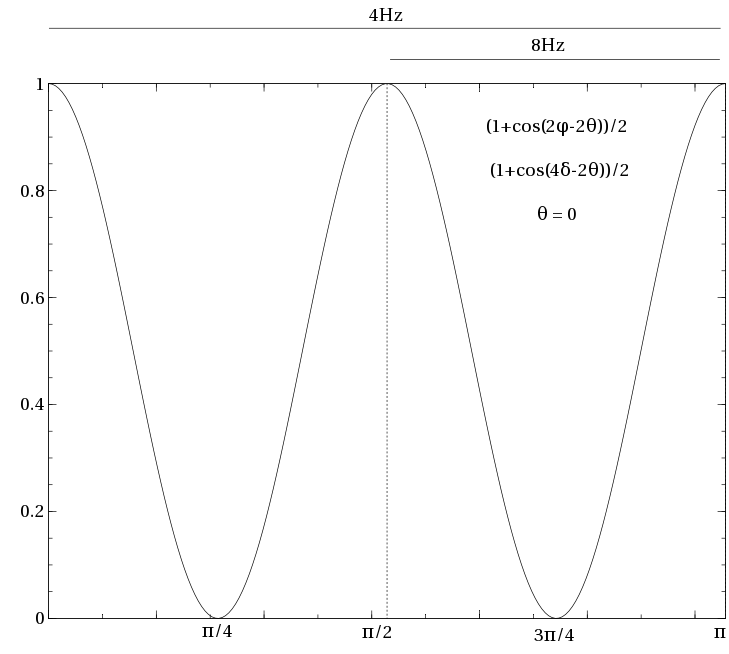
\includegraphics[width=0.7\linewidth]{hwp-modulation.png}
\label{fig:hwpmodulation}
\caption [Attenuation of signal by HWP]{The incoming polarised
  radiation (with a polarised angle, $\theta$, of zero) is attenuated
  by the HWP.  The HWP rotates at 2Hz (through $2\pi$) so we see the
  signal is modulated at 8Hz as the instrument scans at
  8\si{\arcsecond}/s. }
\end{center}
\end{figure}


\begin{figure}[t!]
\begin{center}
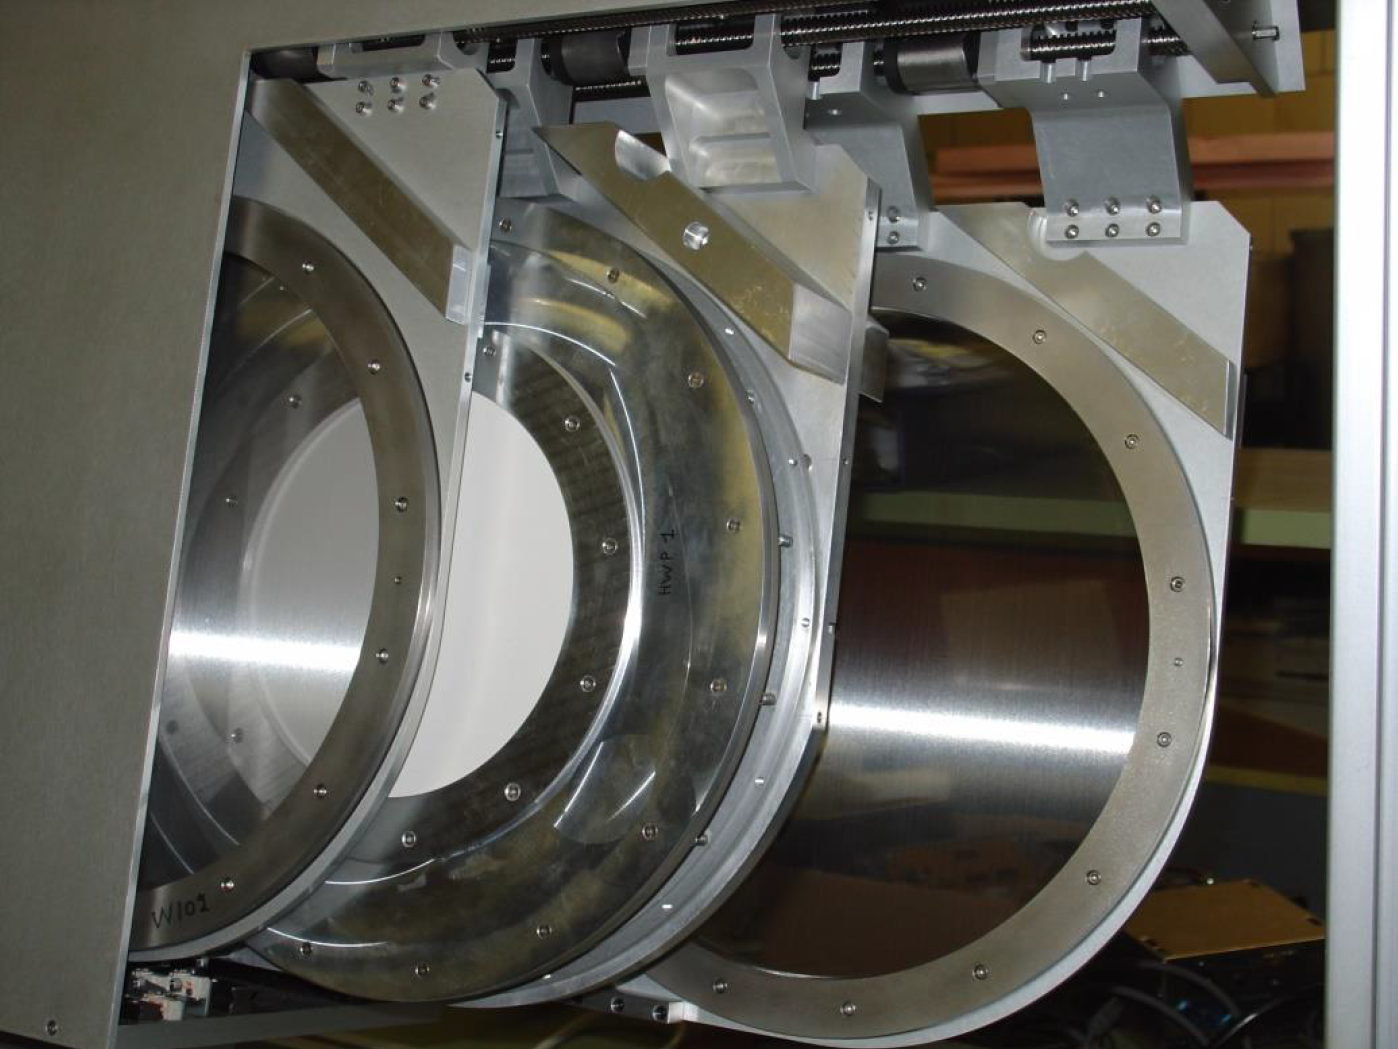
\includegraphics[width=0.7\linewidth]{pol2-three-components.png}
\label{fig:pol2components}
\caption [POL-2 components]{
  The three blades that combine to form POL-2 are partially
  extended showing the two wire grids and the achromatic HWP.
  The two wire grids are the calibrator grid and the analyser grid.
  The rotating HWP is located between these two fixed grids.
  The calibrator grid is only inserted for test purposes.
  Stiffeners can be seen on all three blades. The one for the HWP
  is particularly thick. Their purpose is to reduce vibrations while
  the HWP spins.
}
\end{center}
\end{figure}




\section{Instrumental Polarisation}
\label{sec:ip}

At the angular resolution of JCMT, planets such as Uranus should
appear as unpolarised point sources.  In practice, however, POL-2
observations of such sources exhibit a measurable level of
polarisation - albeit typically less than 1.5\% at 850 $\mu$m. This
is evidence that some part of the incoming astronomical radiation is
being partially polarised by one or more of the components of the
telescope/POL-2/SCUBA-2 that are in the light path. This polarisation
is referred to as "Instrumental Polarisation" (IP).

In order to establish the true Q and U from an astronomical source, it
is necessary to correct for this effect. For the case of a low degree
of polarisation in the incoming radiation and a low degree of IP, the
following is a good approximation for correcting the measurement for
the effects of the IP:

\begin{equation}
Q = Q_{m} - I. ip_{q}
\end{equation}

\begin{equation}
U = U_{m} - I. ip_{u}
\end{equation}

where $Q_{m}$ and $U_{m}$ are the measured values for a single
bolometer sample at some point on the sky. $Q$ and $U$ are the true
(corrected) values, $I$ is the astronomical total intensity at the same
point on the sky (i.e. the total intensity after removal of the sky
and electronic backgrounds) and $ip_{q}$ and $ip_{u}$ are factors that
may vary slowly with focal plane position and/or azimuth and
elevation.

IP correction of a POL-2 map therefore requires a total
intensity map of the same area of the sky to be available. This total
intensity map is referred to as the IP reference map.

Whilst flat mirrors or surfaces will produce a small, constant
polarisation across the beam, curved mirrors and other structures (for
example the secondary mirror supports) will produce more complex
polarisation effects, and these may distort the beam shape.
Side-lobes can often show up with strong (typically 10-20\%)
polarisation but these effects are usually far from the
main-beam. Calculations of typical antenna patterns for symmetrical
Cassegrain antennas have not predicted strong polarisation in the main
beam.

The JCMT IP footprint is stronger than might be expected from the
above considerations above (though typically less than 1.5\% of the
total intensity), and has the following distinctive features:

\begin{enumerate}
\item The polarisation intensity is elevation dependent;
\item There is ellipticity of the beam and it is elevation dependent;
\item The beam is elongated in the horizontal direction.
\end{enumerate}

The dominant source of IP at the JCMT is the woven Goretex membrane,
used as a wind blind.  This membrane introduces both losses and
polarisation. This effect is elevation dependent.


\section{\xlabel{obs_modes}Observing mode}
\label{sec:mmodes}

The standard POL-2 observing mode, POLCV\_DAISY, is a “scan and spin”
mode, in which the telescope is moving continuously in a Daisy-type
pattern while the HWP spins.

The POLCV\_DAISY scan mode is similar to the established Daisy scan
mode routinely used for non-polarimetric SCUBA-2 observations of
point-like or compact sources. However it is slightly altered to allow
for a slower telescope scanning speed.


\begin{figure}[t!]
\begin{center}
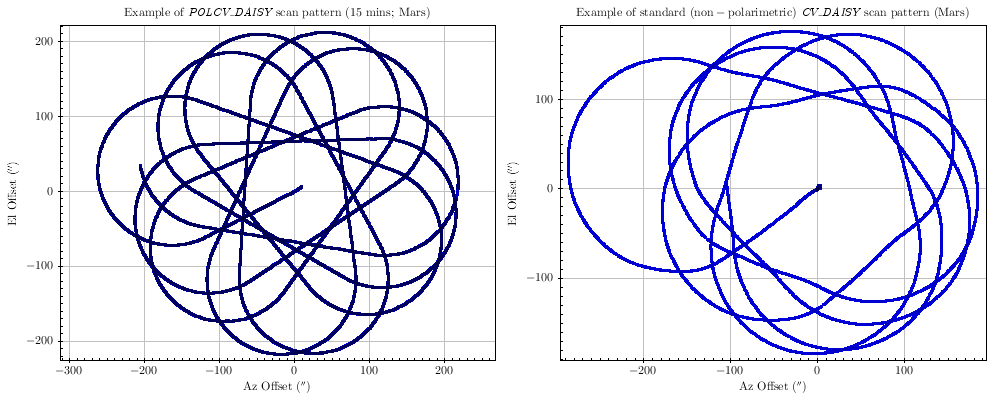
\includegraphics[width=0.9\linewidth]{scan_pattern_daisy_comparison.png}
\label{fig:scancompsrison}
\caption [Scan Pattern Comparison]{Left: Scan pattern from a typical
  SCUBA-2 CV\_Daisy observation. Right: Scan pattern from a POL-2
  Daisy. The standard POLCV\_DAISY scan parameters are given in Table
  \ref{tab:scanpar} }
\end{center}
\end{figure}


The telescope must scan slowly enough to obtain sufficient data at
each point on the sky to allow good $Q$ and $U$ values to be
determined. The current commissioned scan pattern has a size of
200\si{\arcsecond} and a scan speed of 8\si{\arcsecond}/s. The data
reduction splits the data stream into short segments and determines a
pair of $Q$ and $U$ values from each segment.

The length of each such data segment is the time it takes the
telescope to traverse a pixel in the generated map. With the current
scanning parameters this is 0.5 and 0.25 seconds for 850 and
\SI{450}{\micro\metre}, respectively. The modulation generated by any
polarisation is 8 Hz at the current HWP rotation speed (2 Hz).

The standard POLCV\_DAISY scan parameters are given in
Table~\ref{tab:scanpar} and shown in Figure~\ref{fig:scandetail}.

\begin{table}[h!]
\begin{center}
\begin{tabular}{r|l}
\hline
Parameter & Value\\
\hline
Half-wave plate rotation frequency& \SI{2}{Hz}\\
 Antenna scanning speed & 8\si{\arcsecond}/s\\
 R$_{0}$ (map pattern radius)\textdagger
& 133\si{\arcsecond}\\
 R$_{t}$ (turn radius) & 99\si{\arcsecond}\\
 R$_{a}$ (nominal avoidance radius) & 77\si{\arcsecond}\\
\hline
\end{tabular}
\caption{The scan parameters used in the POLCV\_DAISY
  mode. \textdagger This radius is \emph{not} the size of the
  resulting map. }
\label{tab:scanpar}
\end{center}
\end{table}


\begin{figure}[t!]
\begin{center}
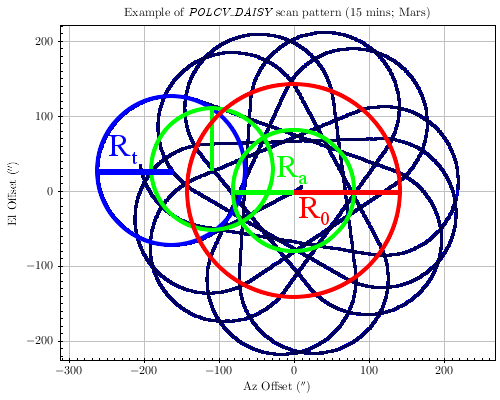
\includegraphics[width=0.6\linewidth]{POLCV_DAISY_schematic_detailed.png}
\caption [Detail of POL-2 Scan Pattern]{Detail of
  POLCV\_DAISY. $R_{0}$ is the map pattern radius, $R_{t}$ the turn
  radius, and $R_{a}$ is the nominal avoidance radius. For more
  details see Table~\ref{tab:scanpar}.}
\label{fig:scandetail}
\end{center}
\end{figure}


\section{The raw data}
\label{sec:rawdata}
SCUBA-2 is the detector for POL-2, and as such, the raw data format of
POL-2 data is the same as a typical SCUBA-2 observation. The sequence
for both observations is:

\begin{enumerate}\itemsep-0.2em
\item Dark noise
\item Flat-field
\item Science scans
\item Flat-field
\end{enumerate}


The \param{SEQ$\_$TYPE} keyword in the FITS header may be used to
identify the nature of each scan.  When you access raw data from the
CADC archive
\htmladdnormallink{http://www3.cadc-ccda.hia-iha.nrc-cnrc.gc.ca/jcmt/}\
you will get all of the files listed above.


Critically the \param{INBEAM} keyword in the FITS header may be used
to identify if POL-2 is in the beam, and hence differentiate between
SCUBA-2 and POL-2 observations.


\begin{tip}
  Use the \Kappa\ command fitslist to see all FITS headers in a
  particular NDF. To obtain a specific header simply use the command
  fitsval:
  \begin{terminalv}
% fitsval s8a20160112_00056_0001.sdf INBEAM
pol
\end{terminalv}
The FITS header information may also be viewed via the \gaia\ View /
FITS header drop-down menu option.
\end{tip}

Shown below is an incomplete list of the raw files for a single
sub-array (in this case s8a) for a short POL-2 observation. The first
and last scans are the flat-field observations,which occur after the
shutter opens to the sky at the start of the observation and closes at
the end (note the identical file size); all of the scans in between
are science scans.


\begin{terminalv}
% ls -lh /jcmtdata/raw/scuba2/s8a/20160112/00056
\end{terminalv}

\begin{terminalv}
-rw-r--r-- 1 jcmtarch jcmt 5.6M Jan 12  2016 s8a20160112_00056_0001.sdf
-rw-r--r-- 1 jcmtarch jcmt 7.9M Jan 12  2016 s8a20160112_00056_0002.sdf
-rw-r--r-- 1 jcmtarch jcmt  25M Jan 12  2016 s8a20160112_00056_0003.sdf
-rw-r--r-- 1 jcmtarch jcmt  25M Jan 12  2016 s8a20160112_00056_0004.sdf
-rw-r--r-- 1 jcmtarch jcmt  25M Jan 12  2016 s8a20160112_00056_0005.sdf
...
-rw-r--r-- 1 jcmtarch jcmt  25M Jan 12  2016 s8a20160112_00056_0025.sdf
-rw-r--r-- 1 jcmtarch jcmt  25M Jan 12  2016 s8a20160112_00056_0026.sdf
-rw-r--r-- 1 jcmtarch jcmt  25M Jan 12  2016 s8a20160112_00056_0027.sdf
-rw-r--r-- 1 jcmtarch jcmt  22M Jan 12  2016 s8a20160112_00056_0028.sdf
-rw-r--r-- 1 jcmtarch jcmt 7.9M Jan 12  2016 s8a20160112_00056_0029.sdf
\end{terminalv}

The SCUBA-2 data acquisition (DA) system writes out a data file every
30 seconds; each of which contains 22\,MB of data. The only exception
is the final science scan which will usually be smaller (7.9\,MB in
the example above), typically requiring less than 30 seconds of data
to complete the observation.

\textbf{Note:} All of these files are written out eight times, once
for each of the eight sub-arrays. It should also be noted that the
POL-2 instrument has not been released from commissioning at 450
$\mu$m.

The main data array in each NDF is a cube, with the first two
dimensions corresponding to bolometer columns and rows within a
sub-array, and the third dimension corresponding to time slice index
(sampled at roughly 200\,Hz).

A standardised file naming scheme is used in which each file name
starts with the sub-array name, followed by the UT date of the
observation in the format \texttt{yyyymmdd}, followed by a five-digit
observation number, followed by the sub-scan number. The name ends
with the standard suffix \texttt{.sdf} used by all Starlink NDF data
files. For instance, the files listed above hold data from the s8a
sub-array for observation 34 taken on 12\textsuperscript{th} January
2016.




\subsubsection*{Units/Calibration}

Raw POL-2 data come in uncalibrated units. The first calibration step
is to scale the raw data to units of pico Watts (pW) by applying the
flat-field solution. This step is performed internally by the SMURF
command calcqu - used to calculate I, Q and U time-streams from the
raw data - but can be done manually when examining the raw data.

If the purpose of a given POL-2 observation is to determine the
percentage polarisations or vector angles within a source/region of
interest then the data may remain in pW. On the other hand, if the
purpose is to establish the absolute polarised intensities then a
value for the Flux Conversion Factor (FCF) is required.

The resulting map may have the FCF applied to convert it into units of
Janskys. As is recommended with SCUBA-2 observing, it is advisable to
check that the FCF value applied to the data is sensible (and must be
done manually). For more details see
\cref{Chapter}{sec:pol2map-fcf}{POL-2 FCFs}.






\newpage
\chapter{\xlabel{pol2_dr}POL-2 Data Reduction - The Theory}
\label{sec:dr}
\section{\xlabel{dataflow}The Data Flow}

POL-2 data reduction is a complex and involved process for which a broad overview is presented first before
the specific details are discussed. It is noted that this same procedure is used whether there is one or 
multiple observation to reduce.

The data reduction process can be broken down into three main steps as shown in Figure \ref{fig:pol2drflow}.

\begin{figure}[t!]
\begin{center}
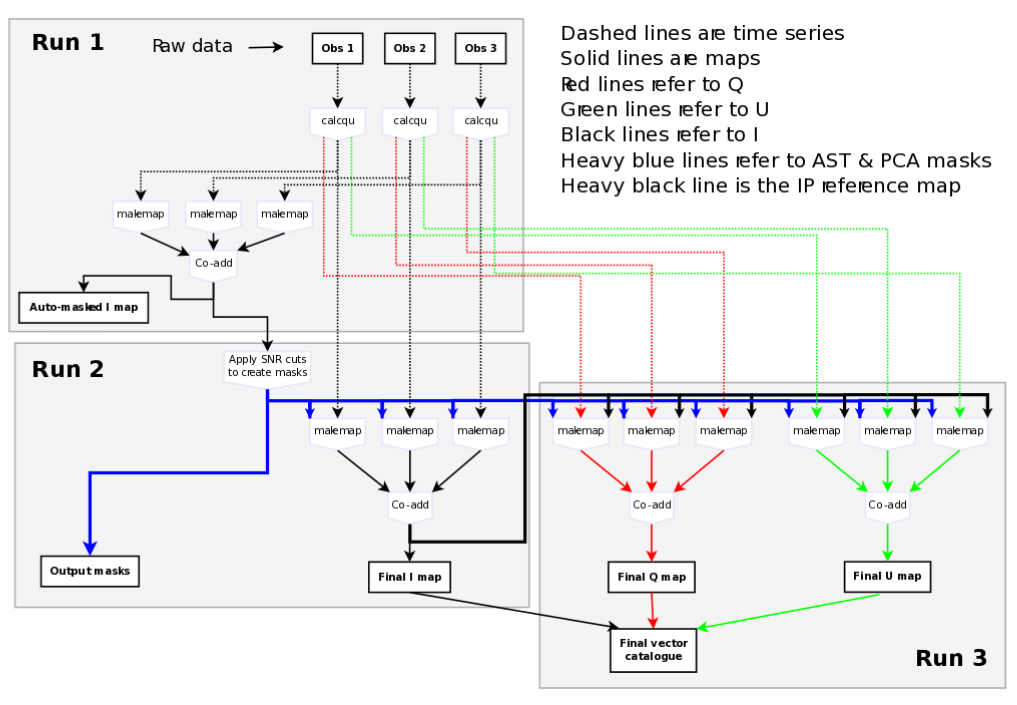
\includegraphics[width=0.95\linewidth]{pol2-dr-flow.png}
\label{fig:pol2drflow}
\caption [POL-2 Data Flow]{
  \small The data flow of the POL-2 data reduction method is
  presented. In this example three POL-2 observations are
  reduced and combined in various stages and combination to
  produce I, Q and U maps.
}
\end{center}
\end{figure}


\subsection*{Step 1}

The inital step of the process (see Run 1 in Figure \cite{fig:pol2drflow}) creates 
an intensity, I, map from the raw data files provided to the reduction routine (see \cref{Chapter}{sec:rundr}). 


\subsubsection*{The process}
The  analysed  intensity values in the raw data time-streams are first converted into Q, U and I time-streams
using smurf:calcqu (these are stored for future use in the directory qudata, specified by the qudir parameter in the example command below). 

The smurf:makemap command is then used to create a separate map from the I time-stream for each observation, using SNR-based “auto-masking” to define the background regions that are to be set to zero at the end of each iteration.  

These maps are stored for future use in the directory maps, specified by the mapdir parameter. Each map has a name of the form:

<UT_DATE>_<OBS_NUM>_<CHUNK_NUM>_imap.sdf

where <CHUNK_NUM> indicates the raw data file at the start of the contiguous chunk of data used to create the map, and is
usually 0003. Each of these maps is compared to the specified reference map (if any) to determine a pointing correction to be applied to the observation in future
2 . If no reference map is supplied, the I map created from the first observation defines the expected source position, and is compared with later maps to determine their pointing corrections.


\subsection*{Step 2}

In the second step of the process (see Run 2 in Figure \cite{fig:pol2drflow}) an improved I map is produced. This improvements come from i) applied relative pointing corrections 


\subsection*{Step 3}



\section{\xlabel{makemap}Makemap}

The POL-2 data reduction builds upon the SCUBA-2 make-map data reduction. The Dynamic Iterative Map-Maker, hereafter just referred to as the map-maker is the tool you will use to produce SCUBA-2 maps, and is implemented by the Smurf makemap command. It performs all pre-processing steps to clean the data, followed by solving for multiple signal components using an iterative algorithm, and binning the resulting time-series data to produce a final science map. 



\cite{smurf}

\section{\xlabel{pca}PCA}


\section{\xlabel{masking}Masking}
A mask is a two-dimensional array which has the same shape and size as the final map, and
which is used to indicate where the source is expected to fall within the map. Bad pixel values
within a mask indicate background pixels, and good pixels values indicate source pixels. Masks
are used for two main purposes:

\begin{enumerate}\itemsep-0.2em
\item To prevent the growth of gradients and other artificial large scale structures within the
map.  For this purpose, the astronomical signal at all background pixels defined by the
mask is forced to zero at the end of each iteration within makemap (except for the final iteration).
\item To prevent bright sources polluting the evaluation of the various noise models (PCA, COM, FLT) used within
makemap. Source pixels are excluded from the calculation of these models.
\end{enumerate}


The pol2map script uses different masks for these two purposes - the “AST” mask and the “PCA” mask. 
The PCA mask is in general less extensive than the AST mask, with the source areas being restricted to the brighter inner regions.
Each of these two masks can either be generated automatically within makemap, or be specified by
a fixed external NDF. 

\section{\xlabel{addingdata}Adding new observations}



\section{\xlabel{tailoredDR}Tailoring your reduction}

\subsection*{variances between POL-2 maps}

MAPVAR is a parameter that controls the variances in the coadded 
I, Q and U maps are formed.

If  MAPVAR is set TRUE, the variances in the coadded I, Q and U maps
are formed from the spread of pixel data values in the individual
observation maps. If MAPVAR is FALSE (the default), the variances in
the coadded maps are formed (as in previous versions of pol2map) by
propagating the pixel variance values created by makemap from the
individual observation maps.

Only use MAPVAR=TRUE if you have enough observations to
make the variances between them meaningful. It's hard to put a lower
limit on it, but it is advised that at a minimum 10 observations.


If you want to test the effect of this option on a field for which you
already have the I, Q and U maps from a set of individual
observations, you can do the following:

\begin{terminalv}
% pol2map in=maps/\* iout=imapvar qout=qmapvar uout=umapvar mapvar=yes \
                   ipcor=no cat=cat_mapvar debias=yes
\end{terminalv}

assuming your I, Q and U maps are in directory "maps". The variances
in imapvar.sdf qmapvar.sdf and umapvar.sdf will be calculated using
the new method, and these variances will then be used to form the
errors in the cat_mapvar.FIT catalogue.




\newpage
\chapter{\xlabel{pol2_dr_running}POL-2 Data Reduction -- Running
  pol2map}
\label{sec:rundr}

The previous chapter, \cref{Chapter}{sec:dr}{POL-2 Data Reduction --
  The Theory}, described how \poltwomap\ produces $I$, $Q$, and $U$ maps from raw
POL-2 data.  It showed that this reduction process----which uses
\poltwomap---comprises three steps.

As with the other Python scripts in \SMURF, it is possible to get more
information about the available parameters by running either:
\begin{terminalv}
% pol2map --help
\end{terminalv}
or the
\begin{terminalv}
% smurfhelp pol2map
\end{terminalv}
command.

\section{\xlabel{how-pol2map}How to use pol2map}

Before running \poltwomap\ directly, it is necessary to ensure that
the \starlink\ environment has been initialised and the \smurf\
package started (see \cref{Section}{sec:starinit}{Initialising
  Starlink} and \cref{Section}{sec:packinit}{KAPPA and SMURF for data
  processing}).

This chapter describes how to run \poltwomap\ firstly to produce an
initial $I$ map; and then again to produce the final $I$, $Q$, and $U$ maps
and a vector catalogue, as described in \cref{Section}{sec:how-step1}{
pol2map -- producing the initial $I$ map}.

To run \poltwomap, values should normally be supplied for the following
command-line parameters\footnote{Note the distinction between
  ``command-line parameters'' that are supplied on the
  \poltwomap\ command line, and ``configuration parameters'' that
  are specified within a configuration file. Values for all
  \emph{configuration} parameters are obtained using a single
  \emph{command-line} parameter called \param{CONFIG}.}, in order to
  produce the initial intensity image. Note that if a parameter description ends
  with a value in square brackets, it is the default value that will be used for
the parameter if no value is supplied on the command line.

\begin{aligndesc}
\item[\texttt{IN}] A list of input NDFs containing raw POL-2 data.
  There are many ways in which the list of files can be supplied, as
  described in the ``\xref{Specifying Groups of
    Objects}{sun95}{se_groups}'' section of \xref{SUN/95}{sun95}{}. The
  easiest of these is to create a simple text file containing the names of the
  raw data files (one per line), and then supply the name of the
  text file, preceded by an up-caret character (\,\texttt{\^{}}\,), as
  the value for parameter \param{IN}. Note that the specified names of the raw
  data files can contain wildcards such as ``$*$'' and ``?''.

\item[\texttt{IOUT}] The name of the NDF in which to store the
  total intensity ($I$) map (in pW) incorporating all supplied observations.
  The supplied file name should either have a file type of
  \texttt{.sdf}, or no file type at all (in which case
  \texttt{.sdf} will be appended to the supplied value). Any existing
  file with the same name will be overwritten.

\item[\texttt{QOUT}] The output NDF in which to return the $Q$ map
  incorporating all supplied observations. This will be in units of
  pW. Null (\texttt{!}) should be supplied if no $Q$ map is required.

\item[\texttt{UOUT}] The output NDF in which to return the $U$ map
  incorporating all supplied observations. This will be in units of
  pW. Null (\texttt{!}) should be supplied if no $U$ map is required.

\item[\texttt{MAPDIR}] The name of the directory in which to place the $Q$,
  $U$, and $I$ maps made from each individual observation supplied via
  \param{IN}, before co-adding them. If null (\texttt{!}) is supplied, the new
  maps are placed in the same temporary directory (chosen automatically)
  as all the other intermediate files, and so will be deleted when the script
  exits (unless the parameter \param{RETAIN} is set to be \texttt{TRUE}). Note
  that these maps are always in units of pW. Each one will contain FITS
  headers specifying the pointing corrections needed to align the map with
  the reference map. [\texttt{!}]

\item[\texttt{QUDIR}] The name of a directory in which to place the $Q$, $U$,
  and $I$ time series generated by \SMURF\ \task{calcqu}, prior to generating
  maps from them. If null (\texttt{!}) is supplied, they are placed in the same
  temporary directory as all the other intermediate files, and so will
  be deleted when the script exits (unless the parameter \param{RETAIN} is
  set to be \texttt{TRUE}). [\texttt{!}]
\end{aligndesc}

Some additional command-line parameters are required when \poltwomap\ is
used for the second time---as discussed in
\cref{Section}{sec:how-step23}{pol2map -- producing the $I$, $Q$, $U$ maps
and catalogue}---to produce the final $I$, $Q$, $U$ maps and vector catalogue\footnote{This
second usage of \poltwomap\ includes both ``Run 2'' and ``Run 3'' in
\cref{Figure}{fig:pol2drflow}{}.}.

\begin{aligndesc}

\item[\texttt{CAT}] The output FITS vector catalogue. No catalogue is
  created if null (!) is supplied. Note that, by default, the $Q$, $U$, and
  $I_{\textnormal{p}}$ values in this catalogue will be in units of mJy/beam. [!]

\item[\texttt{MASK}] Specifies the type of masking to be used within
  \makemap\ (the same type of masking is used to create all three maps---$I$,
  $Q$, and $U$).

\item[\texttt{MASKOUT1}] If a non-null value is supplied for \param{MASKOUT1},
  it specifies the NDF in which to store the AST mask created from the NDF
  specified by Parameter \param{MASK}. Only used if an NDF is supplied for
  Parameter \param{MASK}. [!]

\item[\texttt{MASKOUT2}] If a non-null value is supplied for \param{MASKOUT2},
  it specifies the NDF in which to store the PCA mask created from the NDF
  specified by Parameter \param{MASK}. Only used if an NDF is supplied for
  Parameter \param{MASK}. [!]

\item[\texttt{IPREF}] The total intensity map to be used for IP
  correction. The map must be in units of pW. If the same value is
  supplied for both \param{IOUT} and \param{IPREF}, the output $I$
  map will be used for IP correction. [\texttt{!}]

\item[\texttt{DEBIAS}] \texttt{TRUE} if a correction for statistical bias is to
  be made to percentage polarisation and polarised intensity in the
  output vector catalogue specified by the parameter \param{CAT}. [\texttt{FALSE}]
\end{aligndesc}

The \poltwomap\ command provides many other parameters that may be used to
modify its behaviour in various ways. To see a full list, type

\begin{terminalv}
% pol2map --help
\end{terminalv}


\section{\xlabel{how-step1}pol2map -- producing the initial $I$ map}
\label{sec:how-step1}

As discussed in \cref{Chapter}{sec:dr}{POL-2 Data Reduction -- The
  Theory}, \poltwomap\ must first be run on the raw data to produce an
initial $I$ map.  In this first step:

\begin{terminalv}
% pol2map in=^myfiles.list iout=iauto qout=! uout=! mapdir=maps qudir=qudata
\end{terminalv}

The file \texttt{myfiles.lis} contains a list of the raw data
files to be included in the map, and could (for instance) look like
this:

\begin{terminalv}
% cat myfiles.lis
/jcmtdata/raw/scuba2/s8a/20160125/00043/*
/jcmtdata/raw/scuba2/s8b/20160125/00043/*
/jcmtdata/raw/scuba2/s8c/20160125/00043/*
/jcmtdata/raw/scuba2/s8d/20160125/00043/*
\end{terminalv}

This uses all available data from all four 850\,$\mu$m sub-arrays, for
Observation 43 taken on 25th January 2016\footnote{The input files
  should all be for a single waveband from one or more POL-2
  observations. Users should not mix files from different wavebands and/or
  astronomical regions.}. In addition, the data used in this example
also come from Observations 56 and 59 taken on January 11th 2016 (UT).

\begin{tip}
  An up-caret ( $ \hat{} $ ) is required any time the user is reading in
  a group text file in Starlink. For the map-maker, this includes the
  configuration file (a group of configuration parameters) and the
  list of input files (a group of NDFs \emph{e.g.} \texttt{in= $
    \hat{} $ myfiles.lis}).

  Note that the \poltwomap\ script also invokes the \ \smurf\
  \xref{pol2check}{sun258}{POL2CHECK} command, in order to 
  first ensure that the input files are actually POL-2 files.
\end{tip}

Note that \texttt{qout} and \texttt{uout} are set to null values, as no
$Q$ or $U$ maps are required to be produced during this initial step~1
reduction stage.

The following shows the output from running this initial \poltwomap\
command.

\begin{terminalv}
Logging to file pol2map.log
Calculating Q, U and I time streams from raw analysed intensity data...
   1/3: Processing 116 raw data files from observation 20160125_00043 ...
   2/3: Processing 116 raw data files from observation 20160112_00059 ...
   3/3: Processing 116 raw data files from observation 20160112_00056 ...

>>>>   Making I map from 20160125_00043_0003...

>>>>   Making I map from 20160112_00056_0003...

>>>>   Making I map from 20160112_00059_0003...

Co-adding I maps from all observations:

20160125_00043_0003: Storing pointing corrections of (0.0,0.0) arc-seconds
for future use

20160112_00056_0003: Storing pointing corrections of (1.9,2.8) arc-seconds
for future use

20160112_00059_0003: Storing pointing corrections of (2.1,2.4) arc-seconds
for future use

\end{terminalv}

The files and folders produced by this reduction process are described below.

\begin{aligndesc}
\item[\file{pol2map.log}] A log file containing the output from the
  various \SMURF, \KAPPA\ and \POLPACK\ commands run as part of the \poltwomap\
  command (\poltwomap\ is actually a Python script that runs various other
  Starlink tasks behind the scenes in order to perform the bulk of the work).

\item[\file{qudata/}] A folder containing the $I$, $Q$, and $U$ time-series data
  for each sub array for each observation. Tthese are produced by
  \task{calcqu} (see Section~\cref{Chapter}{sec:calcqu}{CALCQU}.

\item[\file{maps/}] A folder containing the individual $I$ maps from
  each separate observation. These will have names that end with
  \file{$\_$imap.sdf}.

\item[\file{iauto.sdf}] Output total intensity map. The included term ``auto'' is
used to indicate that it was created using an automatically generated
AST mask.

\end{aligndesc}

The output $I$ map, \file{iauto.sdf}, can be opened and viewed with \GAIA.

\begin{figure}[t!]
\begin{center}
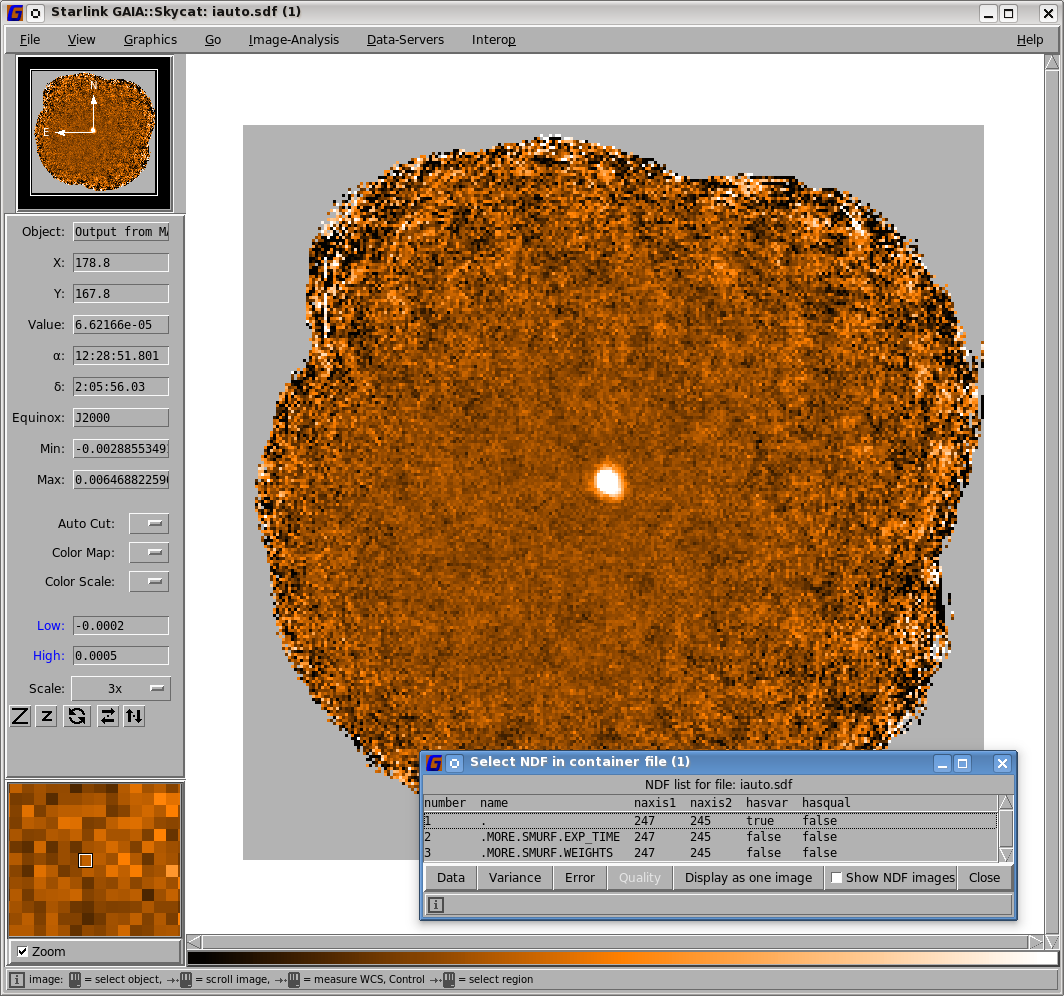
\includegraphics[width=0.8\linewidth]{sc22-gaia-view-iauto.png}
\label{fig:gaia-iauto}
\caption [I map in GAIA]{
  \small The $I$ map, \file{iauto.sdf}, as viewed with \GAIA.
}
\end{center}
\end{figure}

The \file{maps} folder contains the individual $I$ maps from each separate
observation:

\begin{terminalv}
20160112_00056_0003_imap.sdf  20160112_00059_0003_imap.sdf  20160125_00043_0003_imap.sdf
\end{terminalv}

and the \file{qudata} folder contains these files.

\begin{terminalv}
s8a20160112_00056_0003_IT.sdf  s8b20160112_00059_0003_IT.sdf  s8c20160125_00043_0003_IT.sdf
s8a20160112_00056_0003_QT.sdf  s8b20160112_00059_0003_QT.sdf  s8c20160125_00043_0003_QT.sdf
s8a20160112_00056_0003_UT.sdf  s8b20160112_00059_0003_UT.sdf  s8c20160125_00043_0003_UT.sdf
s8a20160112_00059_0003_IT.sdf  s8b20160125_00043_0003_IT.sdf  s8d20160112_00056_0003_IT.sdf
s8a20160112_00059_0003_QT.sdf  s8b20160125_00043_0003_QT.sdf  s8d20160112_00056_0003_QT.sdf
s8a20160112_00059_0003_UT.sdf  s8b20160125_00043_0003_UT.sdf  s8d20160112_00056_0003_UT.sdf
s8a20160125_00043_0003_IT.sdf  s8c20160112_00056_0003_IT.sdf  s8d20160112_00059_0003_IT.sdf
s8a20160125_00043_0003_QT.sdf  s8c20160112_00056_0003_QT.sdf  s8d20160112_00059_0003_QT.sdf
s8a20160125_00043_0003_UT.sdf  s8c20160112_00056_0003_UT.sdf  s8d20160112_00059_0003_UT.sdf
s8b20160112_00056_0003_IT.sdf  s8c20160112_00059_0003_IT.sdf  s8d20160125_00043_0003_IT.sdf
s8b20160112_00056_0003_QT.sdf  s8c20160112_00059_0003_QT.sdf  s8d20160125_00043_0003_QT.sdf
s8b20160112_00056_0003_UT.sdf  s8c20160112_00059_0003_UT.sdf  s8d20160125_00043_0003_UT.sdf
\end{terminalv}


\section{\xlabel{how-step23}pol2map -- producing the $I$, $Q$, $U$ maps and catalogue}
\label{sec:how-step23}

As discussed in \cref{Chapter}{sec:dr}{POL-2 Data Reduction -- The
  Theory}, the I map output from the initial run of \poltwomap\ is used to
derive the final $I$, $Q$, and $U$ maps. If requested, a vector catalogue is
also produced.

The second and third steps of the POL-2 data reduction process can be
run via a single command.

\begin{terminalv}
% pol2map in=qudata/\* iout=iext qout=qext uout=uext mapdir=maps mask=iauto \
          maskout1=astmask maskout2=pcamask ipref=iext cat=mycat debias=yes
\end{terminalv}

The following shows the output from running this second \poltwomap\
command. First, \poltwomap\ produces new $I$ maps for each map, correcting
the position using the correction stored in the old $I$
map\footnote{This correction is found by aligning the old $I$ map with the
\file{iauto.sdf} map.}, and then co-adds all the observations.

\begin{terminalv}
Logging to file pol2map.log
(existing file pol2map.log moved to pol2map.log.1)

Masking will be based on SNR values in 'iauto'.

>>>>   Making I map from 20160112_00056_0003...

   Using pre-calculated pointing corrections of (1.9,2.8) arc-seconds

>>>>   Making I map from 20160125_00043_0003...

   Using pre-calculated pointing corrections of (0.0,0.0) arc-seconds

>>>>   Making I map from 20160112_00059_0003...

   Using pre-calculated pointing corrections of (2.1,2.4) arc-seconds
Coadding I maps from all observations:
\end{terminalv}

As \poltwomap\ continues, the $Q$ and $U$ maps are produced, again with
pointing corrections. This is followed by the creation of the output
vector catalogue.

\begin{terminalv}
>>>>   Making Q map from 20160112_00056_0003...

   Using pre-calculated pointing corrections of (1.9,2.8) arc-seconds

>>>>   Making Q map from 20160125_00043_0003...

   Using pre-calculated pointing corrections of (0.0,0.0) arc-seconds

>>>>   Making Q map from 20160112_00059_0003...

   Using pre-calculated pointing corrections of (2.1,2.4) arc-seconds
Coadding Q maps from all observations:

>>>>   Making U map from 20160112_00056_0003...

   Using pre-calculated pointing corrections of (1.9,2.8) arc-seconds

>>>>   Making U map from 20160125_00043_0003...

   Using pre-calculated pointing corrections of (0.0,0.0) arc-seconds

>>>>   Making U map from 20160112_00059_0003...

   Using pre-calculated pointing corrections of (2.1,2.4) arc-seconds
Coadding U maps from all observations:
Creating the output catalogue: 'mycat'...

45604 vectors written to the output catalogue.
\end{terminalv}


The output of this final run of \poltwomap\ is as follows.

\begin{aligndesc}
\item[\file{pol2map.log}] A log file containing the output from the
  \poltwomap\ command. Note previous log files are moved to a new name
  such as \texttt{pol2map.log.1}.

\item[\file{astmask.sdf}] The AST mask used in the creation
  of the final $I$, $Q$, and $U$ maps.

\item[\file{pcamask.sdf}] The PCA mask used in the creation of the
  final $I$, $Q$, and $U$ maps.

\item[\file{iext.sdf}] The total intensity image, created using the
  external AST and PCA masks described above.

\item[\file{qext.sdf}] The $Q$ map (\emph{i.e} the intensity of the radiation
  linearly polarised in the direction parallel or perpendicular to the
  reference plane), created using an external AST and PCA mask.

\item[\file{maps/}] A folder containing the individual $I$, $Q$, and $U$
  maps from each separate observation. These will have names that end with
  \file{$\_$Imap.sdf}, \file{$\_$Qmap.sdf} or \file{$\_$Umap.sdf}.

\item[\file{uext.sdf}] The $U$ map (\emph{i.e.} the intensity of the radiation
  linearly polarised in the direction $\pm45^{\circ }$ to the reference plane).

\item[\file{mycat.FIT}] The output vector catalogue, containing a
  range of values derived by \poltwomap\ for each pixel contained within
  the $I$ map.

\end{aligndesc}


\begin{figure}[t!]
\begin{center}
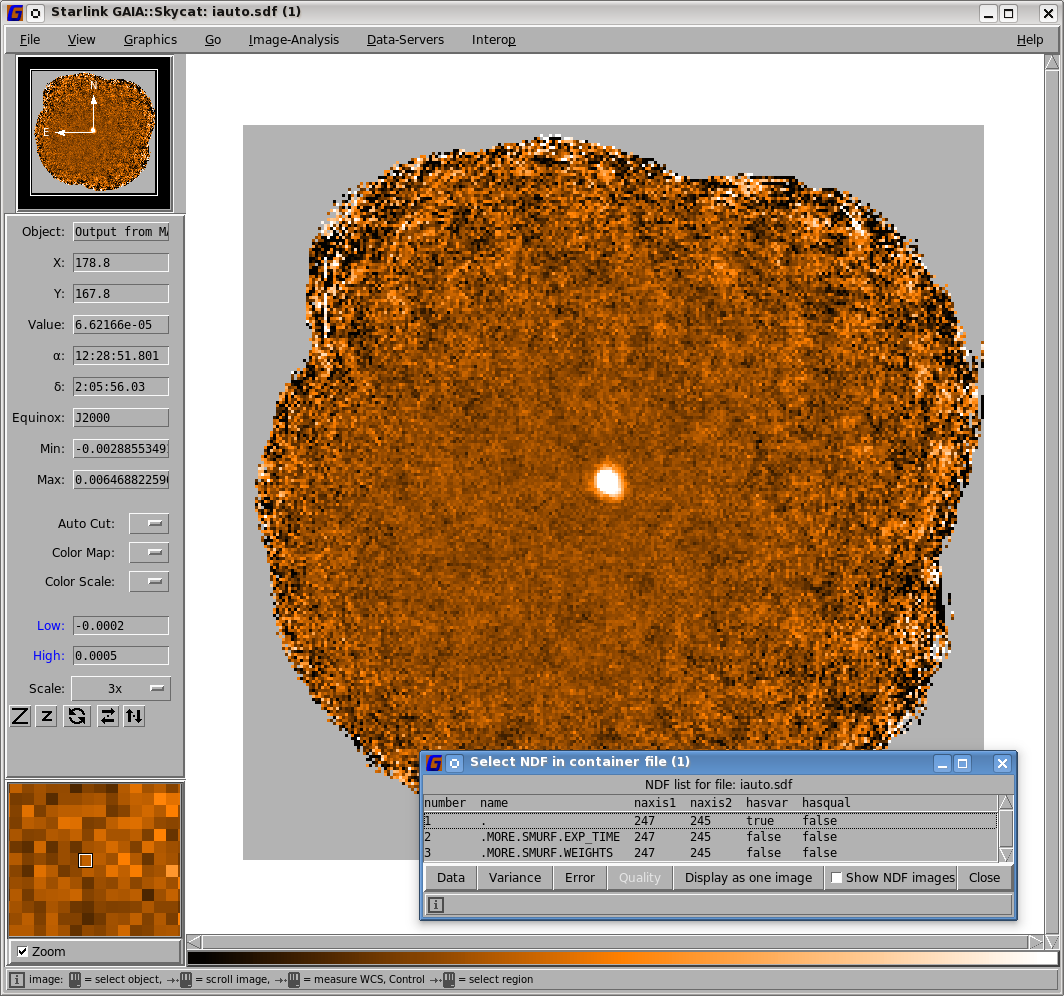
\includegraphics[width=0.46\linewidth]{sc22-gaia-view-iauto.png}
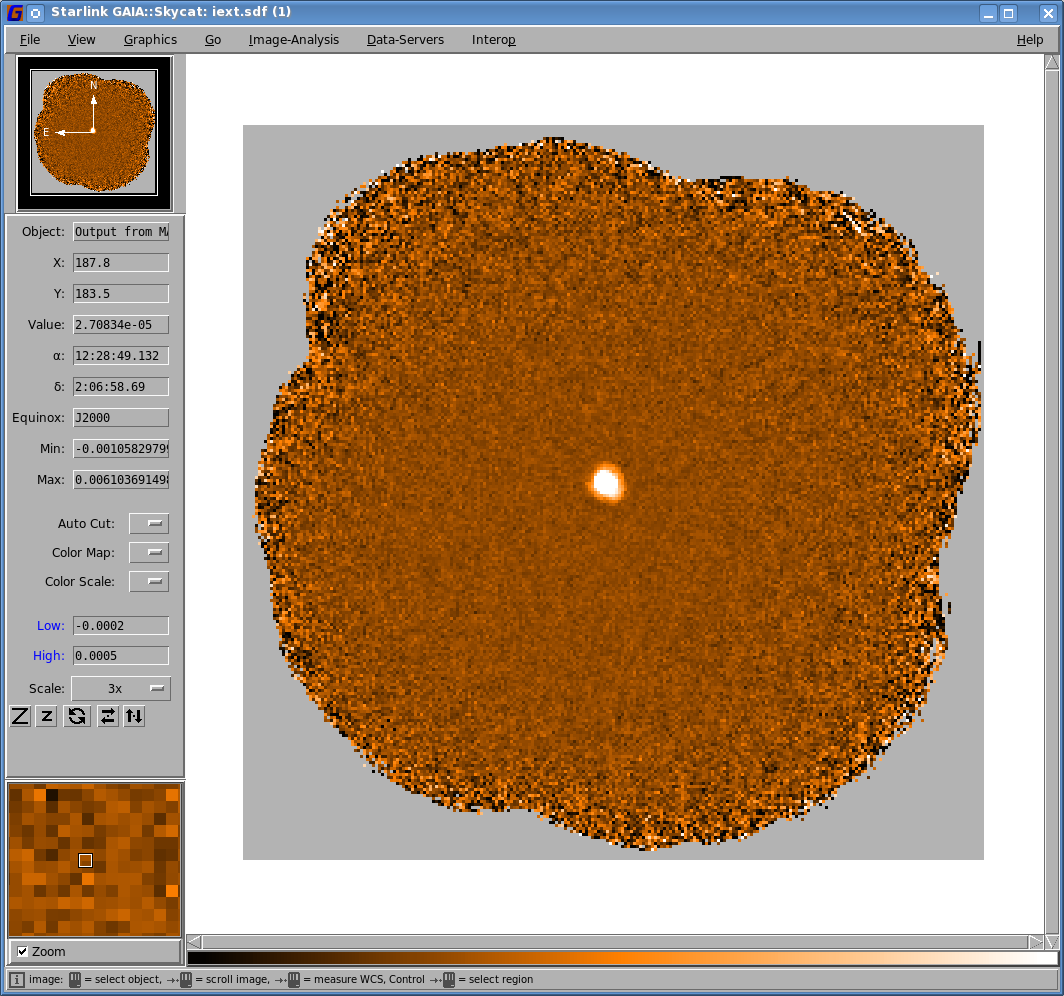
\includegraphics[width=0.46\linewidth]{sc22-gaia-view-iext.png}
\label{fig:gaia-iext}
\caption [Final I map in GAIA]{
  \small Left: $I$ map, \file{iauto}, as produced by the automask on the first pass
         of \poltwomap. Right: Final $I$ map, \file{iext}, as viewed with \GAIA.
         The flatter background is due to the increase in \param{pca.pcathresh}.
}
\end{center}
\end{figure}


\begin{figure}[t!]
\begin{center}
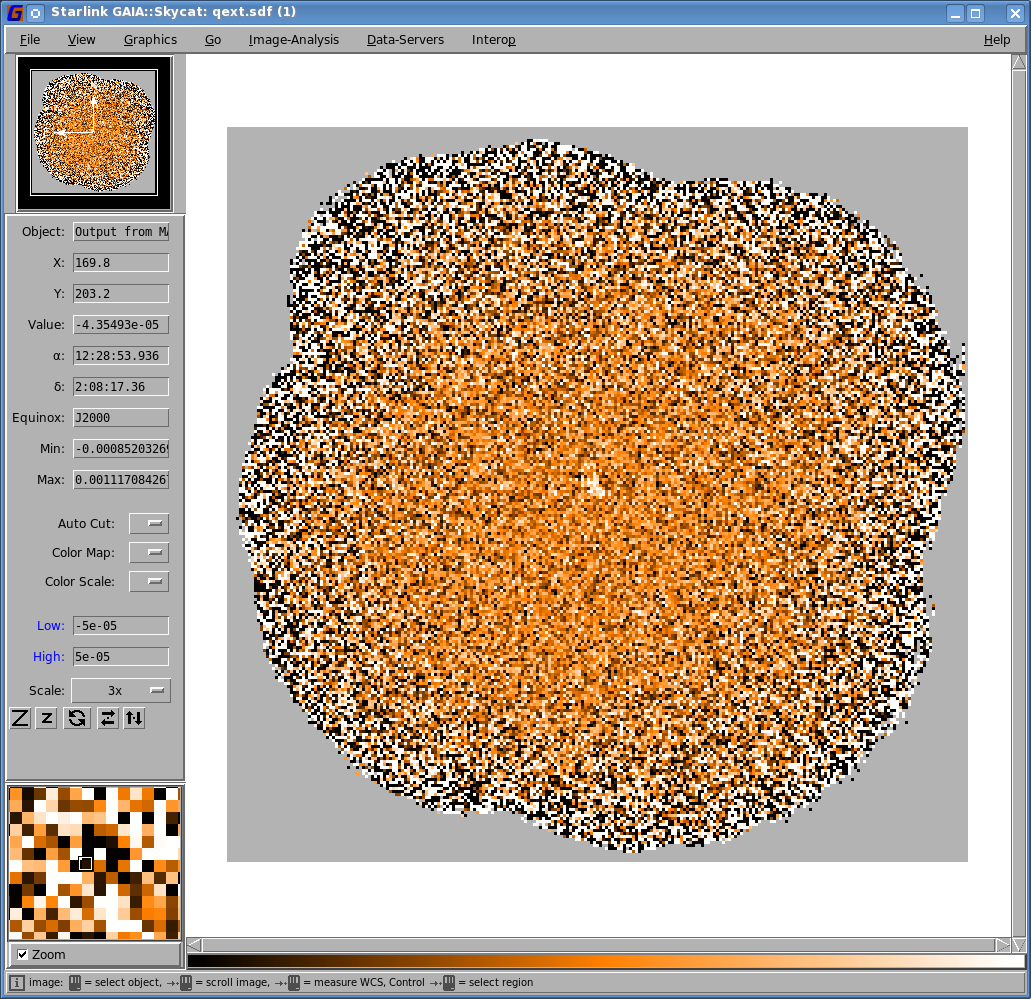
\includegraphics[width=0.46\linewidth]{sc22-gaia-view-qext.png}
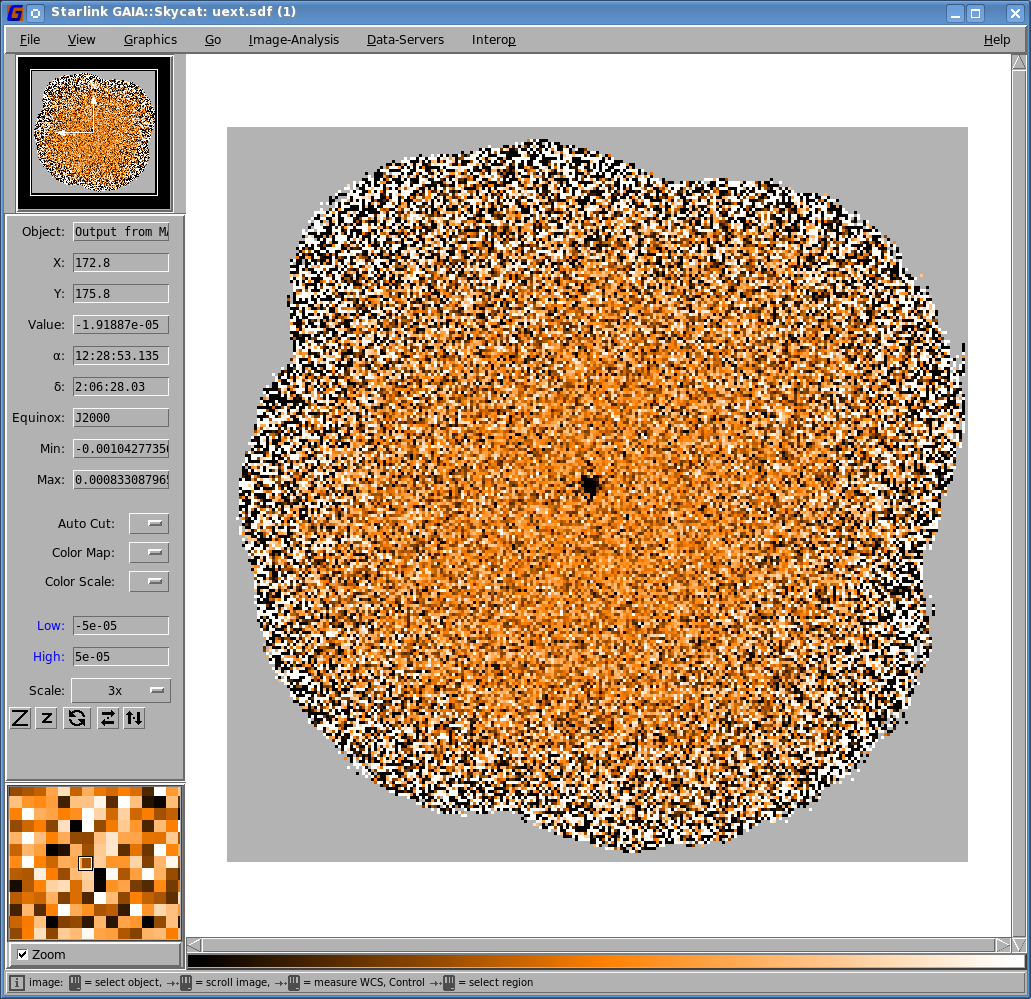
\includegraphics[width=0.46\linewidth]{sc22-gaia-view-uext.png}
\label{fig:gaia-qext-uext}
\caption [Q and U maps in GAIA]{
  \small Left: $Q$ map, \file{qext.sdf}. Right: $U$ map \file{uext.sdf}, as viewed with \GAIA.
}
\end{center}
\end{figure}



The maps folder now contains individual $Q$ and $U$ maps, alongside the
existing $I$ maps listed below.

\begin{terminalv}
20160112_00056_0003_Imap.sdf  20160112_00059_0003_Imap.sdf  20160125_00043_0003_Imap.sdf
20160112_00056_0003_Qmap.sdf  20160112_00059_0003_Qmap.sdf  20160125_00043_0003_Qmap.sdf
20160112_00056_0003_Umap.sdf  20160112_00059_0003_Umap.sdf  20160125_00043_0003_Umap.sdf
20160112_00056_0003_imap.sdf  20160112_00059_0003_imap.sdf  20160125_00043_0003_imap.sdf
\end{terminalv}




\section{\xlabel{vector-cat}Output vectors from pol2map}



The output vector catalogue contains a range of values derived by
\poltwomap\ for each pixel contained within the I map. Intensity values and
errors in the
catalogue are expressed in units of mJy/beam.  If desired, it is possible
to switch the catalogue to units of pW by using \texttt{Jy=no} on the \poltwomap\
command line.  The columns are listed below.

\begin{aligndesc}
\item[\texttt{X}] Pixel coordinate at the centre of the pixel
\item[\texttt{Y}] Pixel coordinate at the centre of the pixel
\item[\texttt{RA}] RA coordinate at the centre of the pixel
\item[\texttt{Dec}] Dec coordinate at the centre of the pixel
\item[\texttt{I}] Total intensity
\item[\texttt{DI}] Error in $I$
\item[\texttt{Q}] Stokes $Q$ parameter
\item[\texttt{DQ}] Error in $Q$
\item[\texttt{U}] Stokes $U$ parameter
\item[\texttt{DU}] Error in $U$
\item[\texttt{P}] Percentage polarisation
\item[\texttt{DP}] Error in $P$
\item[\texttt{ANG}] Angle of polarisation
\item[\texttt{DANG}] Error in ANG
\item[\texttt{PI}] Polarised intensity ($I_{\textnormal{p}}$)
\item[\texttt{DPI}] Error in polarised intensity
\item[\texttt{AST}] Integer values that indicate if the corresponding vector position is inside the AST mask. If the vector is outside the mask, the corresponding column for the mask will have a blank/null value. Vectors that are inside a mask will have a non-zero integer value for the corresponding column. Each ``island'' within a mask (i.e. a contiguous group of source pixels) will have a different integer value assigned, starting at 1. All vectors within an island  are assigned the integer value of the island. 
\item[\texttt{PCA}] Contains integer values that indicate if the corresponding vector position is inside the PCA mask. Value conventions are the same as for the \texttt{AST} column (above).
\end{aligndesc}


\section{\xlabel{pol2fcf}POL-2 FCFs}
\label{sec:pol2map-fcf}

Inserting POL-2 in front of SCUBA-2 reduces the throughput to SCUBA-2.
POL-2 is not a perfect polarimeter. Its wire grid absorbs and scatters incoming
signal so the modulation amplitude is lower than for a perfect polarimeter.
In addition cross polarization and depolarization decreases the modulation
amplitude without decreasing the power in the transmitted signal. The first
type of inefficiencies can be measured by comparing normal SCUBA-2 maps with
and without the polarimeter inserted. Such observations have been done on Uranus,
Mars and Jupiter. The second type of losses can be measured with a source of know polarization.

To convert POL-2 data to astronomical units such as mJy/beam a Flux Conversion
Factor, FCF, must be applied to the data. For POL-2, the FCFs are quoted in terms of
the non-polarimetric SCUBA-2 FCFs.

POL-2 FCFs are now applied automatically within \poltwomap\ when catalogue columns
in mJy/beam are required by the user, i.e. if the \poltwomap\ parameter \texttt{JY} is set
to \texttt{TRUE} (the default option). The current version of \poltwomap\ uses the new,
revised POL-2 FCFs for \SI{850}{\micro\metre} and \SI{450}{\micro\metre}.

\section{\xlabel{tweaking}Changing pixel size in pol2map}
\label{sec:pol2map-pixelsize}

Inevitably, as with unpolarised SCUBA-2 data reduction, users will sometimes find it
necessary to fine-tune the \poltwomap\ reduction process for specific situations.

The bin size within the final vector catalogue is controlled by the
\param{BINSIZE} parameter in the \SMURF\ \poltwomap\ command.

\begin{terminalv}
% pol2map binsize=12
\end{terminalv}

Changing the catalogue bin size in this way does not change the pixel
size of the maps created \poltwomap. Instead, the maps are binned up
to the requested bin size before the catalogue is created. There is
another parameter, called \param{PIXSIZE}, which controls the map pixel
size, but it is usually advisable to leave this at its default value. This is
because the map pixel size can affect the behaviour of the iterative algorithm
used to create maps.








\newpage
\chapter{\xlabel{pol2_image}POL-2 Image Display}
\label{sec:display}

\section{\xlabel{gaia}GAIA}

The \starlink\ package \gaia\ can be used to inspect the results of the data reduction.
To plot the output vector catalogue onto the final total intensity map
first open up the I map in gaia:

\begin{terminalv}
% gaia iext.sdf
\end{terminalv}


Then in the main Gaia window, select the drop-down menu option Image Analysis /
Polarimetry toolbox…. This should launch a new toolbox window entitled
GAIA: Polarimetry. From this window, use the drop-down menu option
File / Open to load the file mycat.FIT. This should then populate the lower part of the
window with the contents of this polarimetry catalogue file.
Each of the vectors in this file will be automatically overlaid on the main image window
(see figure \ref{fig:gaia-plot-vectors1}).

\begin{figure}[t!]
\begin{center}
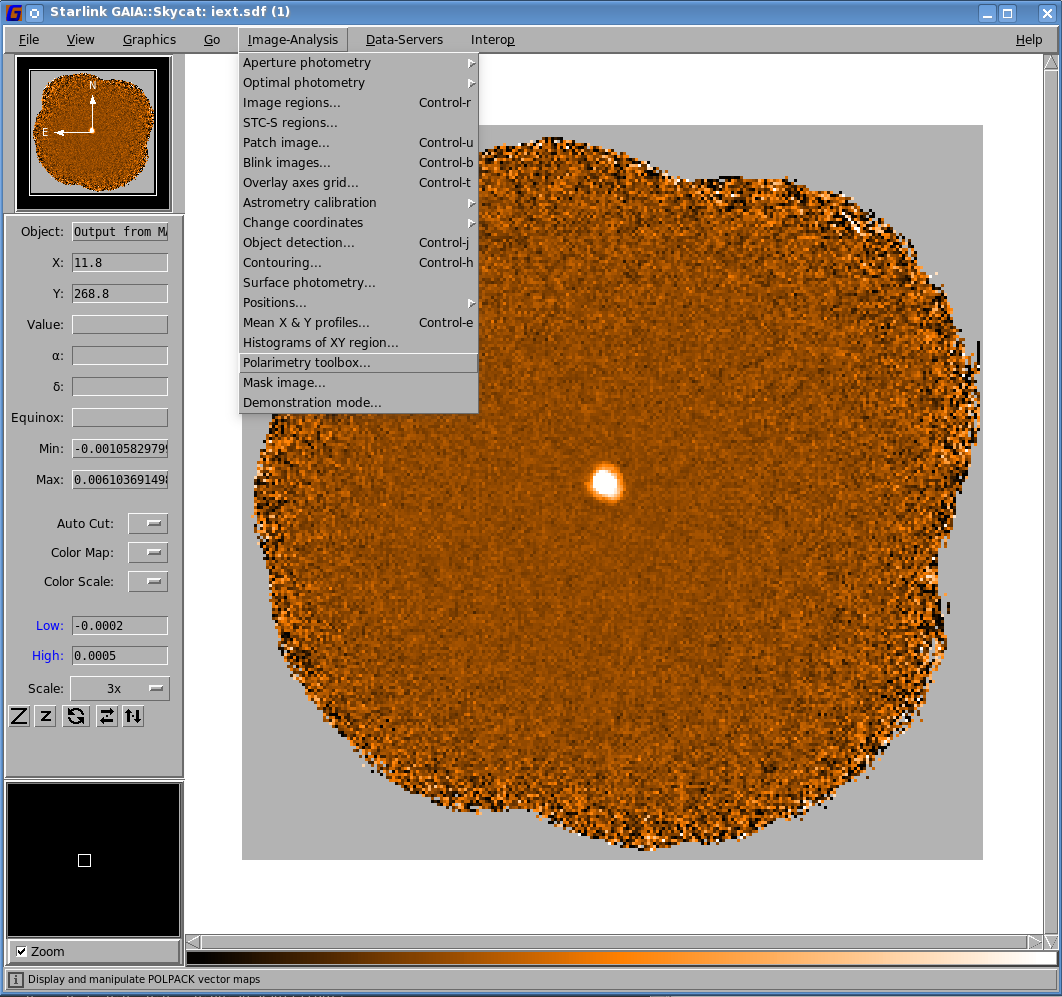
\includegraphics[width=0.46\linewidth]{sc22-gaia-plot-vectors-1.png}
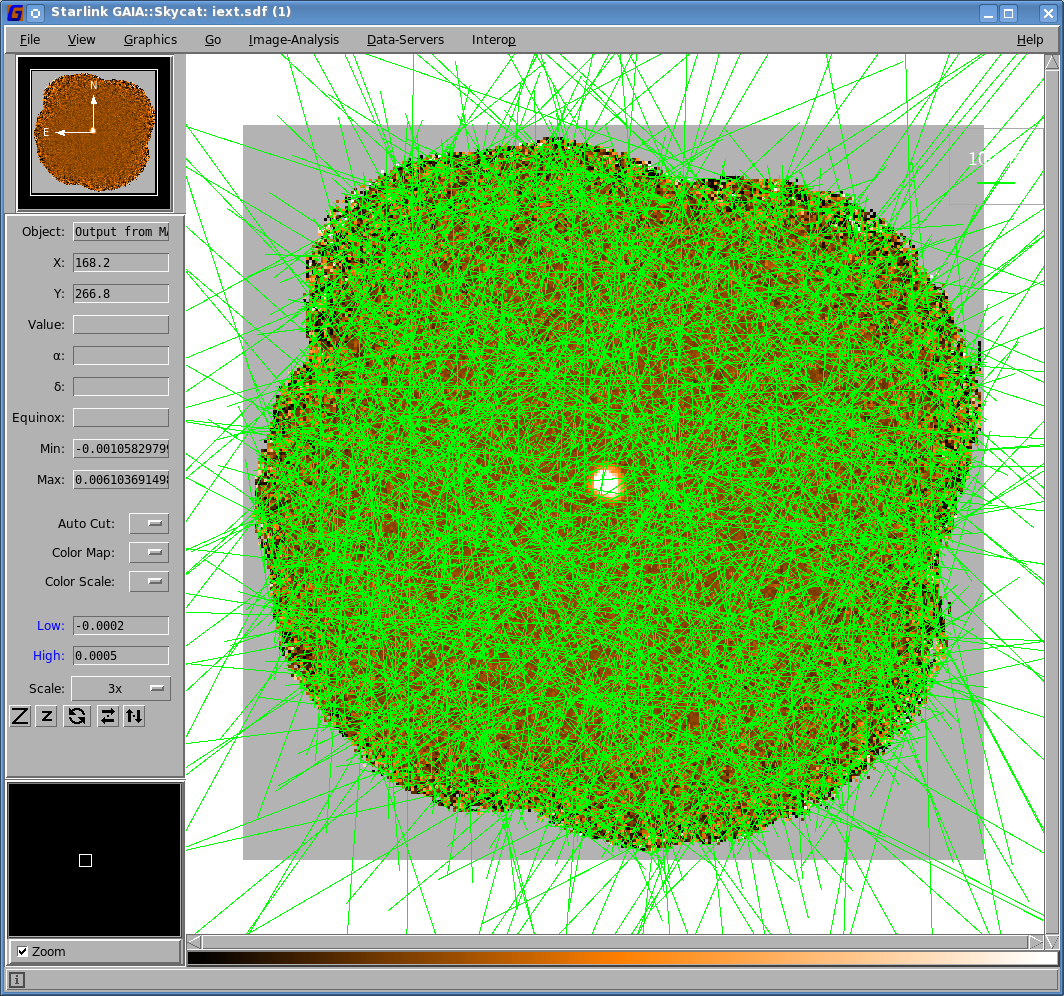
\includegraphics[width=0.46\linewidth]{sc22-gaia-plot-vectors-3.png}
\label{fig:gaia-plot-vectors1}
\caption [Over Plotting Vectors in GAIA]{
  \small Left: Opening up the polarimetry tool box in GAIA. Right: The initial POL-2
vectors overplotted in GAIA.
}
\end{center}
\end{figure}

In order to filter the number of overlaid vectors down to a more useful number and size,
various options in the GAIA: Polarimetry window can be used. First, select the Rendering
tab on the left hand side. This will reveal a panel that will indicate which quantities
are currently being used for the vector overlays. In this case, the Vector length is taken
from the P column of the table, and the Vector angles are taken from the ANG column.

Currently the figure has too many vectors to be scientifically meaningful. To filter
out most of the extraneous vectors, click on the Selecting tab, and set the Expression
field to be the following:

\begin{terminalv}
$I/$DI<10
\end{terminalv}

\emph{Ensure you press return after entering in the above expression}.

The above expression selects the data points in the polarimetry table which have an
associated total intensity (column I) less than 10 times the
associated error value for that intensity (column DI). To remove all of these
extraneous vectors, either press control-X or use the drop-down menu option Edit / Cut.
This should leave just a small number of vectors clustering around the target object.

\begin{figure}[t!]
\begin{center}
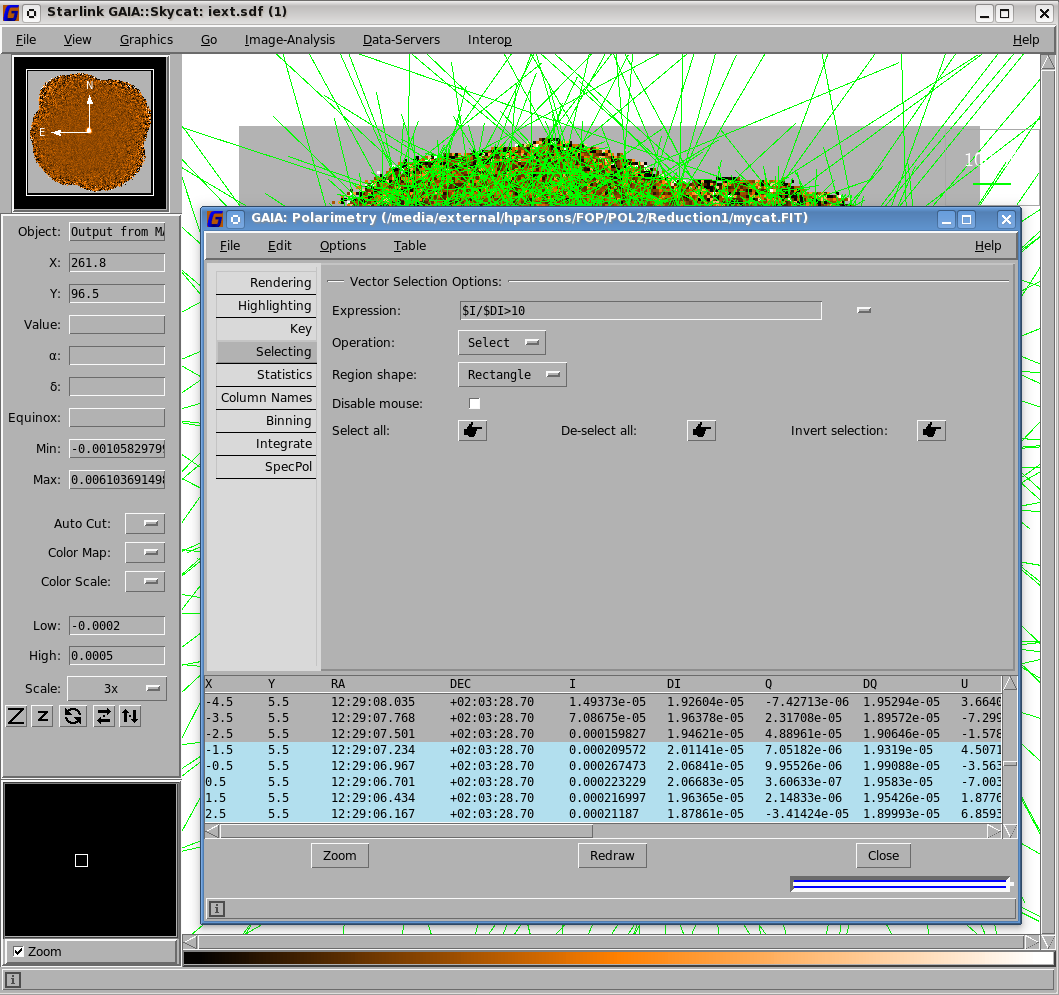
\includegraphics[width=0.46\linewidth]{sc22-gaia-plot-vectors-4.png}
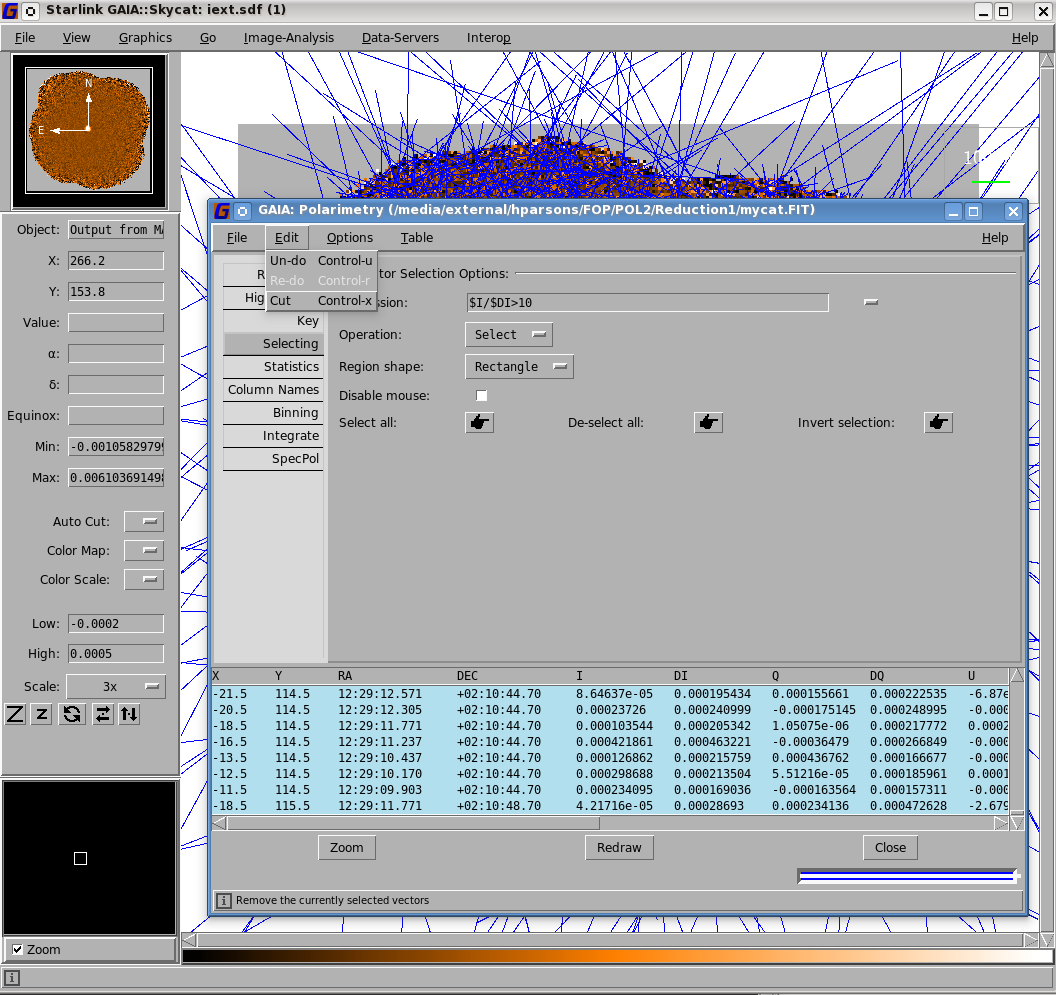
\includegraphics[width=0.46\linewidth]{sc22-gaia-plot-vectors-6.png}
\label{fig:gaia-plot-vectors2}
\caption [Selecting Vectors in GAIA]{
  \small Left: specifying vectors to display via the expression \$I/\$DI$>$10. This will only plot
vectors with an 850 micron intensity signal-to-noise ratio grater than 10 in GAIA. To ensure this is selected
ensure you press the carriage return after entering the expression.
}
\end{center}
\end{figure}

Zooming in on the central region of the map, it can already be seen that the level of vector ordering
(and hence polarization) is quite low (see figure \ref{fig:gaia-plot-vectors3}). If needed it is
possible to change the scaling by selecting the Rendering tab in the GAIA: Polarimetry
window, and increasing the vector scale.


\begin{figure}[t!]
\begin{center}
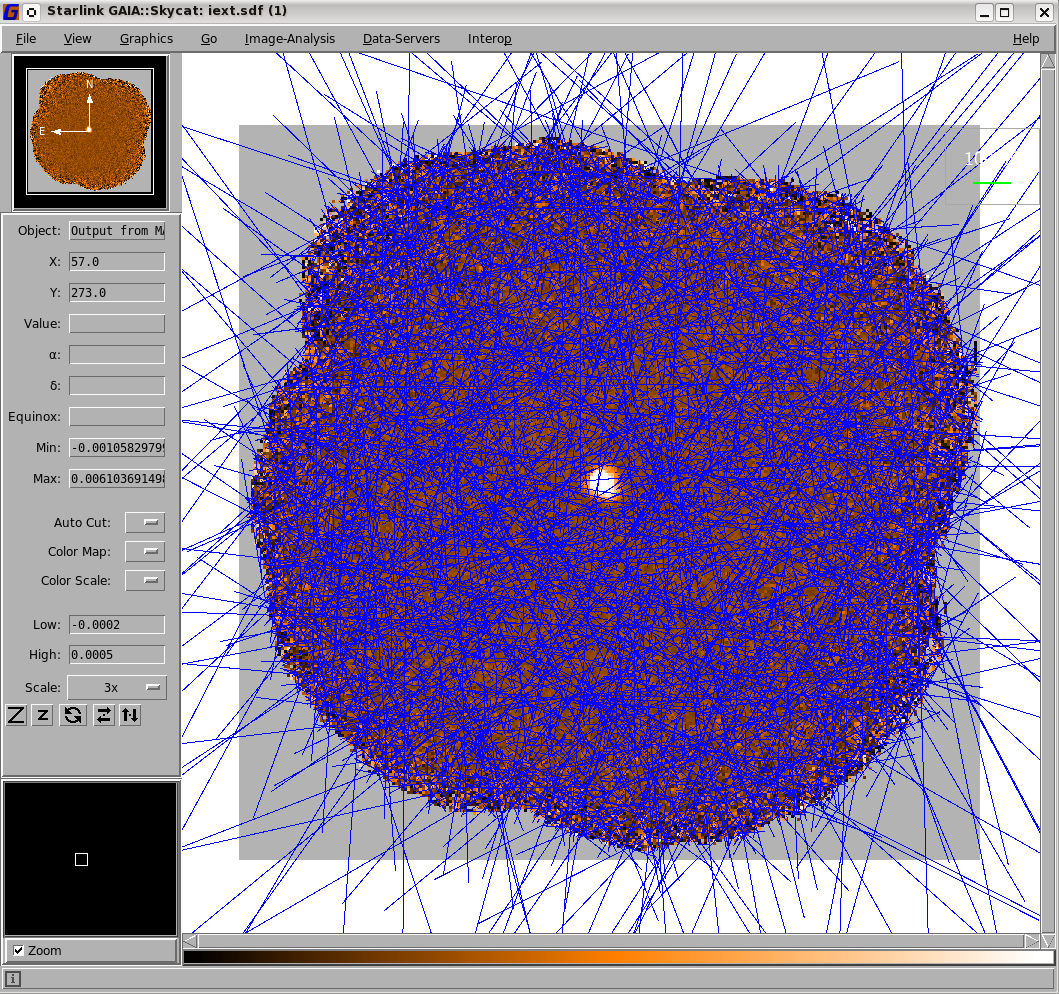
\includegraphics[width=0.44\linewidth]{sc22-gaia-plot-vectors-5.png}
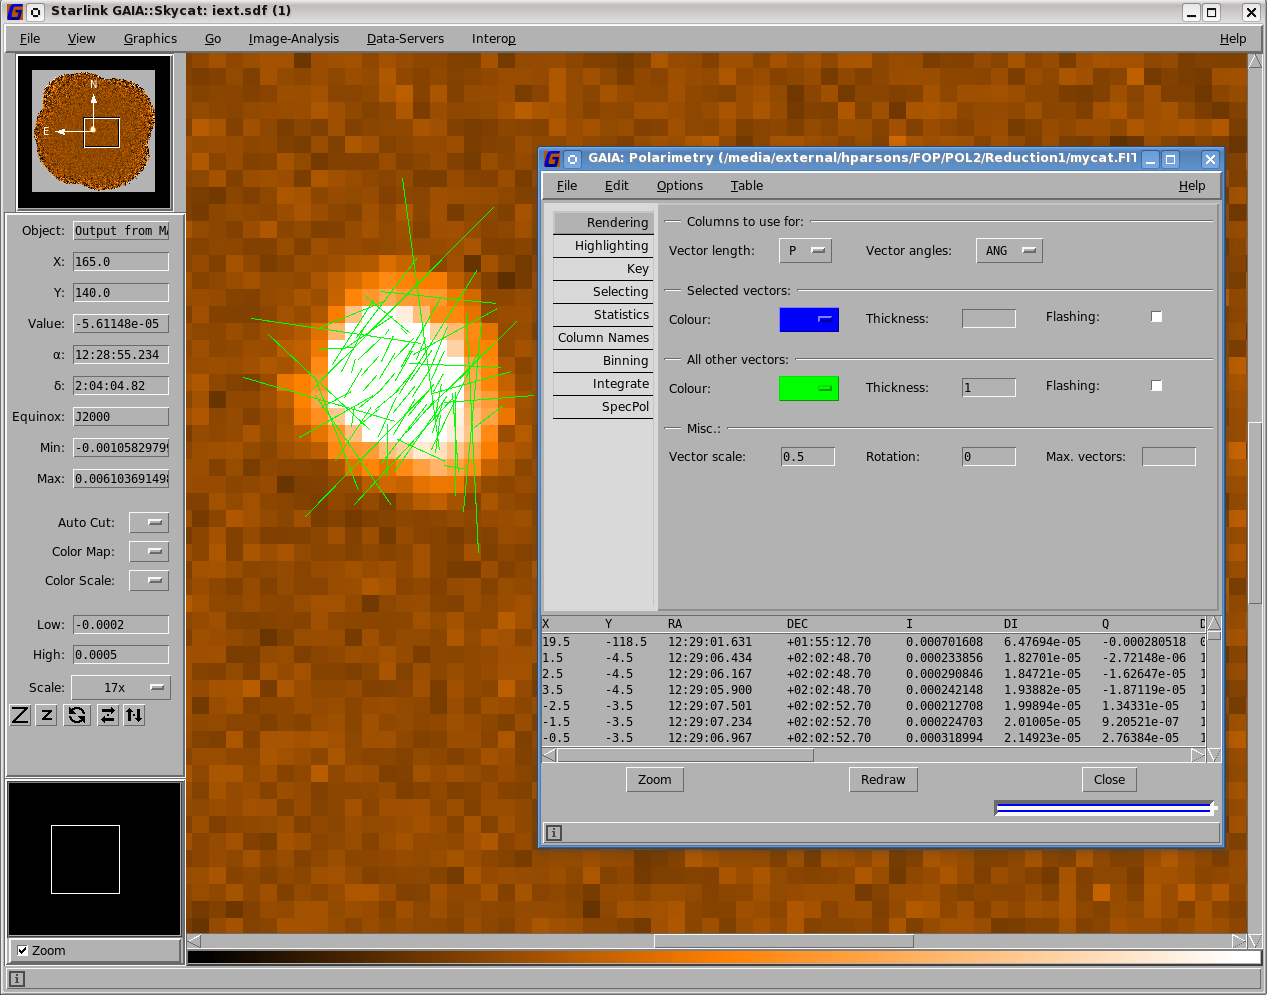
\includegraphics[width=0.52\linewidth]{sc22-gaia-plot-vectors-7.png}
\label{fig:gaia-plot-vectors3}
\caption [Over Plotting Vectors in GAIA]{
  \small Left: Selected vectors are marked in blue in this example, Right: after removal of selected
vectors all that remains are the vectors on the regions where \$I/\$DI$>$10.
}
\end{center}
\end{figure}


\section{\xlabel{kappa}KAPPA and polpack}

It is possible to use \Kappa\ and polpack to create POL-2 plots.

\begin{terminalv}
% kappa
% polpack
\end{terminalv}

Note that in the following examples you will need to ensure that only the
vectors you intend to plot are included in the file mycat.FIT.

There are two main ways to do this - either by saving the output catalogue
from GAIA or using the starlink package \cursa to manipulate the catalogue you produced.
to use cursa simply run:

\begin{terminalv}
% cursa
\end{terminalv}

then to select the vectors of interest:

\begin{terminalv}
% catselect catin=mycat.FIT catout=selcat.FIT norejcat seltyp=e "expr='i>10*di'"
\end{terminalv}

it is also possible to crop images using catselect, by using the expression command. 
In this example we use only pixels above -10 on the y axis.

\begin{terminalv}
% catselect catin=mycat.FIT catout=selcat.FIT norejcat seltyp=e "expr='i>10*di and y>-10'"
\end{terminalv}




\begin{tip}
For a better font on pgplot postscript devices, set the
following environment variable. For more info, see

http://pipelinesandarchives.blogspot.com/2015/02/better-fonts-in-postscript-output-from.html

\begin{terminalv}
setenv PGPLOT_PS_FONT Times
\end{terminalv}

Graphics-related attributes that can be set are described at:
http://starlink.eao.hawaii.edu/docs/sun95.htx/sun95se28.html

and the coordinate system attributes that can be set are
described at:

http://starlink.eao.hawaii.edu/docs/sun95.htx/sun95se27.html
\end{tip}



\subsection{\xlabel{kappa-example1} Example 1 - a vector map with no background}
\label{section:kappa-example1}

In this section we create an output file: plot1.pdf from the input catalogue mycat.FIT

Select postscript graphics device, writing to file plot1.ps

\begin{terminalv}
gdset plot1.ps/acps
\end{terminalv}

For convenience, create a text file holding the main plotting style for polplot.

\begin{terminalv}
% cat sty
colour = black
drawtitle=0
format(1)=hms
format(2)=dms
\end{terminalv}

Likewise, create a text file holding the style for the vector length key

\begin{terminalv}
% cat ksty
colour = black
drawtitle=0
\end{terminalv}


Plot the vector map (the \texttt{vscale} arameter controlls the vector
scale, and the \texttt{keyvec} parameter controls the length of the
vector used as the key. There are many other parameters that can be used
to control the behaviour of \texttt{polplot} - see the \polpack manual - SUN/223.

\begin{terminalv}
% polplot selcat.FIT  style=^sty keystyle=^ksty vscale=20 keyvec=20
\end{terminalv}

Convert to PDF and remove blank margins (if required).

\begin{terminalv}
% ps2pdf plot1.ps temp.pdf
% pdfcrop temp.pdf plot1.pdf
\end{terminalv}


\begin{figure}[t!]
\begin{center}
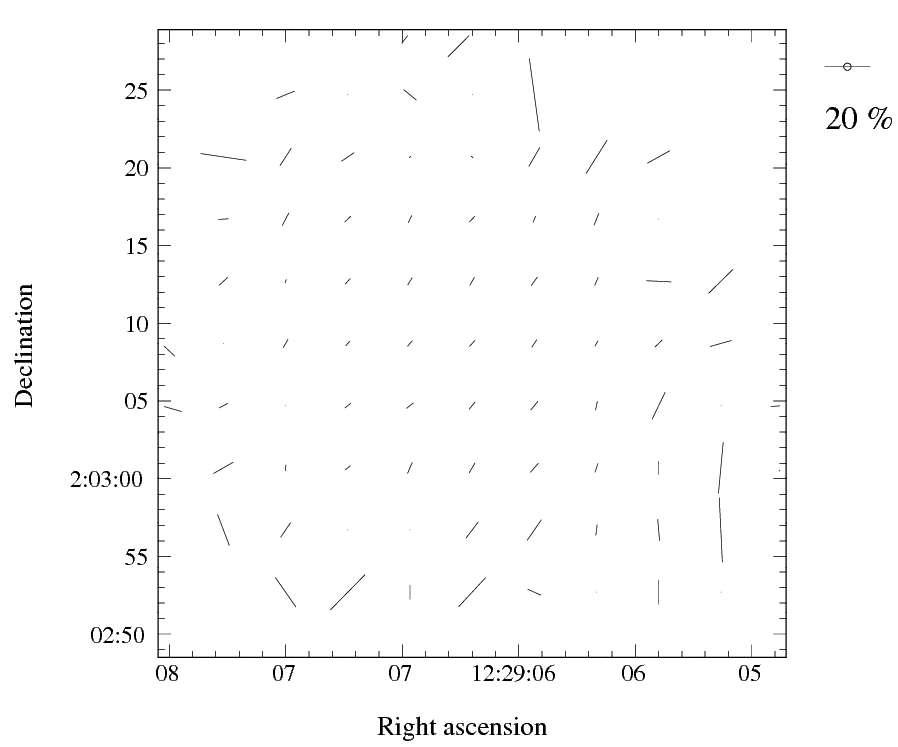
\includegraphics[width=0.75\linewidth]{sc22-kappa-plots-plot1.png}
\label{fig:kappa-plot1}
\caption [Vector map with polplot]{
  \small Result from Example 1: Producing a vector map with no background using polplot. 
}
\end{center}
\end{figure}

\subsection{\xlabel{kappa-example2} Example 2 - a vector map over a contour map}
\label{section:kappa-example2}


In this section we create an output file: plot2.pdf from the input catalogue mycat.FIT

\begin{terminalv}
% gdset plot2.ps/acps
\end{terminalv}

Setting up the main plotting style for contour and polplot

\begin{terminalv}
% cat sty
colour = black
colour(curves)=red
width(curves)=3
drawtitle=0
format(1)=hms
format(2)=dms
\end{terminalv}


Produce the contour map

\begin{terminalv}
% contour iext\(0~150,0~200\) mode=perc percentiles=\[88,90,92,94,96,98\] style=^sty key=no
\end{terminalv}


Modify the above style for the vector map to produce black vectors

\begin{terminalv}
% cat vsty
^sty
colour(curves)=black
\end{terminalv}


The style for the vector length key


\begin{terminalv}
% cat ksty
colour=black
width=3
drawtitle=0
\end{terminalv}

Plot the vector map over the contour map. The vectors and
contours are aligned automatically in sky coordinates.


\begin{terminalv}
% polplot selcat.FIT axes=no clear=no style=^vsty keystyle=^ksty vscale=20 keyvec=20
\end{terminalv}

Convert to PDF and remove blank margins (if required).

\begin{terminalv}
% ps2pdf plot2.ps temp.pdf
% pdfcrop temp.pdf plot2.pdf
\end{terminalv}

\begin{figure}[t!]
\begin{center}
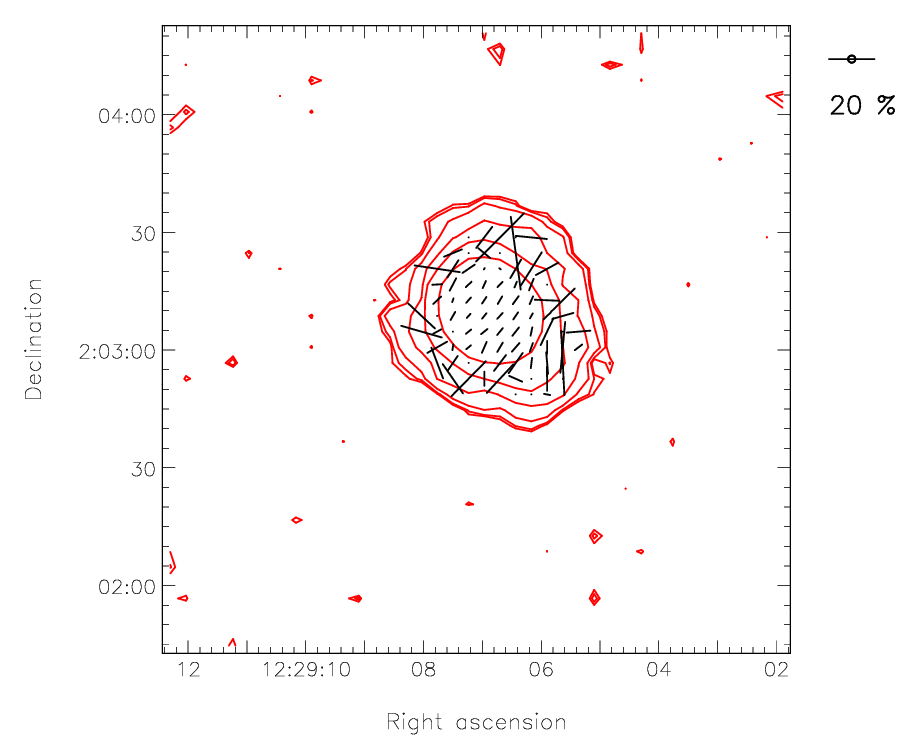
\includegraphics[width=0.75\linewidth]{sc22-kappa-plots-plot2.png}
\label{fig:kappa-plot2}
\caption [Vector map with contour map in polplot]{
  \small Result from Example 1: Producing a vector map over a contour map. 
}
\end{center}
\end{figure}

\subsection{\xlabel{kappa-example2} Example 3 - a vector map over a negative image}
\label{section:kappa-example3}


In this section we create an output file: plot3.pdf from the input catalogue mycat.FIT

\begin{terminalv}
% gdset plot3.ps/acps
\end{terminalv}


Ensure we use a monochrome colour table for the image

\begin{terminalv}
% lutgrey
\end{terminalv}


#  The main plotting style for display and polplot

\begin{terminalv}
% cat sty
colour = black
drawtitle=0
format(1)=hms
format(2)=dms
\end{terminalv}


Use a square root-ish function to reduce the dynamic range in the map (so
that we can see structure in the faint bits without blowing out the
bright bits).

\begin{terminalv}
maths "'((ia+0.0003)/0.14)**0.2'" ia=iext out=tmp1
\end{terminalv}


Display the negative image, using a reduced range of colours
(pens) so that the brightest regions are grey rather than black.
This means the black vectors can still be seen over the bright
regions.

\begin{terminalv}
% display tmp1\(5~150,0~200\) mode=perc percentiles=\[2,98\] style=^sty \
        low=0.4 high=1.0
        penrange=\[0.4,1.0\]
\end{terminalv}


Modify the above style for the vector map to produce wider vectors

\begin{terminalv}
% cat vsty
^sty
width(curves)=3
\end{terminalv}


The style for the vector length key

\begin{terminalv}
% cat ksty
colour=black
width=3
drawtitle=0
\end{terminalv}


Plot the vector map over the contour map. They are aligned automatically with the map.

\begin{terminalv}
% polplot selcat.FIT axes=no clear=no style=^vsty keystyle=^ksty vscale=20 keyvec=20
\end{terminalv}


Convert to PDF and remove blank margins (if required).

\begin{terminalv}
% ps2pdf plot3.ps temp.pdf
% pdfcrop temp.pdf plot3.pdf
\end{terminalv}


\begin{figure}[t!]
\begin{center}
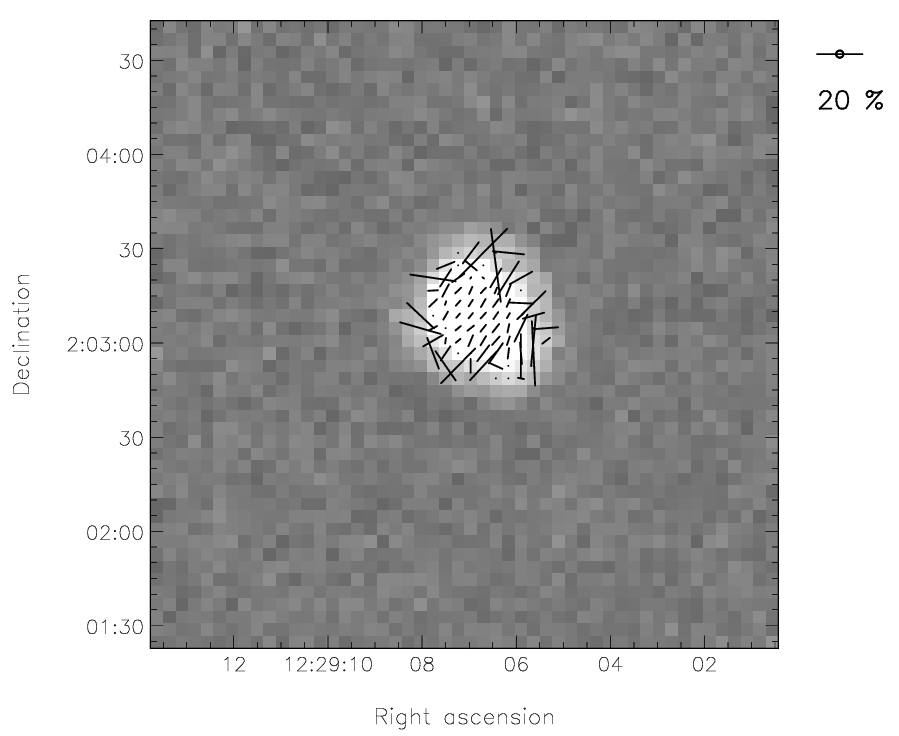
\includegraphics[width=0.75\linewidth]{sc22-kappa-plots-plot3.png}
\label{fig:kappa-plot3}
\caption [Vector map with negative image in polplot]{
  \small Result from Example 1: Producing a vector map over a negative image. 
}
\end{center}
\end{figure}



\newpage
\chapter{\xlabel{pol2_advanced}POL-2 -- Advanced Data Reduction}
\label{sec:advanced}


The \poltwomap\ tool for reducing POL-2 data was originally released for
general science community use several years ago. The fact that its
development remains ongoing directly reflects the continuing advances
made at the cutting edge of POL-2 data reduction and analysis.

This advanced section of the POL-2 data reduction documentation aims
to provide users with additional tools and options with which to refine their
individual POL-2 data reduction processes.

For further ideas, see \cref{Section}{sec:tailoredDR}{Tailoring a reduction}.

\section{\xlabel{addingdata}Adding new observations}

If a user receives additional data after an initial POL-2 reduction of a partial dataset,
then it is almost always easier (and the process more robust) for a user to simply
re-run the reduction process ''from scratch'' for the whole, augmented dataset.
Despite the associated additional processor time cost, therefore, users are generally
recommended to adopt this approach, rather than to attempt to combine new
observations with pre-existing \poltwomap\ reduction products.

For completeness, however, this section describes the six-step process of
combining data for one or more new POL-2 observations into existing $I$, $Q$,
and $U$ maps and vector catalogue created by an earlier run of \poltwomap.
\begin{enumerate}

\item Create a text file listing all the existing auto-masked $I$ maps
  for individual observations stored in the directory specified by
  Parameter \param{MAPDIR}, and then add in the raw data files for the new
  observations. The auto-masked $I$ maps have names that end in
  \file{$\_$imap.sdf}.

\begin{terminalv}
% ls maps/*imap.sdf > infiles.list
% ls rawdata/*.sdf  >> infiles.list
\end{terminalv}


\item Create a new auto-masked, co-added $I$ map including the new
  observation. The \xref{calcqu}{sun258}{CALCQU} and \makemap\ commands
  will be run on the new
  data and the resulting maps combined with the existing maps derived
  from the older observations to create the new map:

\begin{terminalv}
% pol2map in=^infiles iout=iauto_new qout=! uout=! mapdir=maps \
     qudir=qudata
\end{terminalv}


\item A decision needs to be taken as to whether to re-create all the
  externally masked maps using external masks defined by the new
  auto-masked map. This will be the case if the auto-masked map has
  been changed significantly by the addition of the new
  observation. To do this, it is necessary to compare the old and new
  masks. The old masks should have been created earlier using the
  \param{MASKOUT1} and \param{MASKOUT2} parameters (see Step~3 in
  \cref{Section}{sec:dr}{POL-2 Data Reduction -- The Theory}). To
  create the new masks that would be generated from the new
  auto-masked map, use this command:

\begin{terminalv}
% pol2map  in=^infiles iout=! qout=! uout=! mapdir=maps mask=iauto_new \
     maskout1=astmask_new  maskout2=pcamask_new
\end{terminalv}

\item Decide if the addition of the new data has changed the masks
  significantly. This involves comparing \file{astmask.sdf} and
  \file{astmask$\_$new.sdf} (and also \file{pcamask.sdf} and
  \file{pcamask$\_$new.sdf}).


\item If the mask has changed significantly and all observations need
  to be reprocessed using the new mask, or if \task{skyloop} is being used,
  remove the existing externally masked maps so that they will be re-created by
  the next invocation of \poltwomap.  Note that this will increase the length of
  time taken by Step~6 enormously.

  Ensure that the new auto-masked co-add is used in place of the old one, in order to
  define any new masks needed in future:

\begin{terminalv}
% rm mapdir/*Qmap.sdf mapdir/*Umap.sdf mapdir/*Imap.sdf
% mv iauto.sdf iauto_old.sdf
% mv iauto_new.sdf iauto.sdf
\end{terminalv}

\item Re-create the necessary externally masked maps and co-adds, and
  then create the new vector catalogue:

\begin{terminalv}
% pol2map in=qudata/\* iout=iext_new qout=! uout=! mapdir=maps \
     mask=iauto
% pol2map in=qudata/\* iout=! qout=qext_new uout=uext_new mapdir=maps \
     mask=iauto ipref=iext_new cat=mycat_new debias=yes
\end{terminalv}
\end{enumerate}


\section{\xlabel{pixelsize}Experimenting with pixel sizes}

Currently,the default map pixel size is 4\si{\arcsecond} at both
850 and \SI{450}{\micro\metre}. The pixel size is controlled by the
\param{PIXSIZE} parameter in the \smurf\ \poltwomap\ command:

\begin{terminalv}
% pol2map pixsize=12
\end{terminalv}


The following four-step example shows how to investigate the impact of
changing pixel size.  In this example, 12\si{\arcsecond}
pixels and 7\si{\arcsecond} pixels are compared.

\begin{enumerate}
\item Begin with an auto-masked total-intensity map from the raw
  data. For instance:

\begin{terminalv}
% pol2map in=^myfiles.list iout=iauto12 pixsize=12 qout=! uout=! \
     mapdir=maps12 qudir=qudata
\end{terminalv}


\item Create AST and PCA masks with 12\si{\arcsecond} pixels from the
  \file{iauto12.sdf} file:


\begin{terminalv}
% pol2map in=qudata/\* iout=! qout=! uout=! mapdir=maps12 mask=iauto12 \
     maskout1=astmask12 maskout2=pcamask12
\end{terminalv}

\item Create masks with 7\si{\arcsecond} pixels by resampling the
  12\si{\arcsecond} masks created at Step~2. This is done using the
  \Kappa\ \xref{\task{sqorst}}{sun95}{SQORST} command:

\begin{terminalv}
% sqorst  mode=pixelscale pixscale=\'7,7,7E-05\' in=astmask12 out=astmask7
% sqorst  mode=pixelscale pixscale=\'7,7,7E-05\' in=pcamask12 out=pcamask7
\end{terminalv}

\item Create the 7\si{\arcsecond} externally masked $I$, $Q$, and $U$ maps
  using the above 7\si{\arcsecond} masks (note the \texttt{mask}
  parameter value is enclosed in single \emph{and} double quotes).

\begin{terminalv}
% pol2map in=qudata/\* iout=iext7 qout=qext7 uout=uext7 masktype=mask \
                  mask="'astmask7,pcamask7'" mapdir=maps7 ipref=iext7  \
                  cat=cat7 debias=yes
\end{terminalv}
\end{enumerate}

\begin{tip}
  Using larger pixels usually produces slower convergence, and so the
  above process will take longer than usual---be patient!

  Using larger pixels can sometimes encourage smooth blobs and other
  artificial features to appear in the map. The \file{iauto12.sdf} file
  should be examined to check that it does not have such artificial
  features.

  Check the masks (\file{astmask12.sdf} and \file{pcamask12.sdf}) to make sure they
  look reasonable.

  It is usually advisable to leave \param{PIXSIZE} at its default value
  and instead use the \param{BINSIZE} parameter to control the bin size in
  the vector catalogue---see \cref{Section}{sec:pol2map-pixelsize}{Changing pixel size in pol2map}).
\end{tip}

\section{\xlabel{IPerror}Investigating systematic error in IP}


The error on the IP is reported to be of the order of 0.5\%.  It is
possible to investigate the effects of the systematic error in IP by
creating maps using the upper and lower limits on the IP value. The
\task{makemap} configuration parameter called \xparam{IPOFFSET}{ipoffset}
can be used to conduct such an investigation. To use it, run \poltwomap\ twice,
as follows:

\begin{terminalv}
% pol2map config="ipoffset=-0.25"
% pol2map config="ipoffset=0.25"
\end{terminalv}

This will produce maps using the upper and lower IP limits (a range of
0.5\%). If \poltwomap\ has already been run on POL-2 data, then a file will
already exist that was created using the mean IP (the mean IP is used
if \param{ipoffset} is omitted from the configuration value, or the
configuration parameter itself is omitted).

%\section{\xlabel{simulations}Simulated data}


\section{\label{sec:wcscopy}Adding WCS information back into a vector catalogue}
Vector catalogues produced by \poltwomap\ contain information about World Coordinate
Systems (WCS) in two different forms:

\begin{enumerate}
\item The catalogue contains ``RA'' and ``Dec'' columns that hold the sky position
(FK5, J2000) of each vector, in radians.
\item The catalogue header contains a Starlink ``WCS FrameSet'' which defines
(amongst other things) the projection from pixel coordinates within
the $I$, $Q$, and $U$ mosaics, to RA and Dec. This FrameSet is used by Starlink software, together
with the pixels coordinates stored in the ``X'' and ``Y'' columns, to determine
the RA and Dec of each vector. The WCS FrameSet also defines the polarimetric
reference direction used by the $Q$, $U$, and ANG values. See
``\xref{Using World Co-ordinate Systems}{sun95}{se_wcsuse}''
within \xref{SUN/95}{sun95}{} (the \KAPPA\ manual) for more information on
the ways in which Starlink software handles WCS information.
\end{enumerate}

Starlink software such as \polpack, \Kappa, and \gaia\ rely on the WCS
FrameSet for all WCS-related operations (drawing annotated axes, aligning
data sets, \emph{etc}). Thus, problems are likely to arise if the WCS FrameSet
is removed from the vector catalogue. This could happen if (for instance)
inappropriate software is used to process an existing catalogue, creating a
new output catalogue. Under such circumstances, the WCS FrameSet might
not be copied to the output catalogue, causing subsequent WCS-related
operations to fail. It is safe to use \POLPACK, \KAPPA, \GAIA\ and
\xref{\textsc{Cursa}}{sun190}{}), as all these packages copy the WCS
FrameSet to any new output catalogues. Unfortunately, the popular
\topcat\ catalogue browser (see
\url{http://www.starlink.ac.uk/topcat/}) and the STILTS package
(\url{http://www.starlink.ac.uk/stilts/}) upon which it is based, do
\emph{not} copy the WCS FrameSet to any output catalogues.

For this reason, \POLPACK\ contains a command that can be used to copy the
WCS FrameSet from one catalogue to another.  For example: a user creates
the catalogue \file{mycat.FIT} using \poltwomap, uses \textsc{Topcat}
to remove low signal-to-noise vectors, an then saves the results to a new catalogue
called \file{selcat.FIT}. The WCS FrameSet would then be missing from \file{selcat.FIT},
and so it would be necessary to copy it back into place again from the original catalogue
file, \file{mycat.FIT}. To do this, the ``\xref{polwcscopy}{sun223}{POLWCSCOPY}''
command can be used:

\begin{terminalv}
% polwcscopy in=selcat ref=mycat out=selcat2
\end{terminalv}

This would create a third catalogue \file{selcat2.FIT}, which would be a copy of
\file{selcat.FIT}, but with the WCS information inherited from \file{mycat.FIT}.



\section{\xlabel{vectorerrorremodelling}Re-modelling the error estimates in a POL-2 vector catalogue}


If the \texttt{MAPVAR=YES} option is used when running the \smurf\ \poltwomap\ script, the I, Q and U error estimates in the resulting vector catalogue will be based on the spread of pixel values at each point on the sky in the I, Q and U maps made from individual observations. Thus, if 20 observations are processed by \poltwomap\ to create a vector catalogue, then each I, Q or U error estimate in the vector catalogue will be based on the spread of 20 independent measurements of I, Q or U.  Even though 20 observations is a lot of POL-2 data, 20 is still a fairly small number from which to produce an accurate estimate of the error. Consequently, it is usual to see a large level of random ``noise'' on the error estimates, as in the following example, which shows the total intensity (I) error estimates taken from a 12\si{\arcsecond} vector catalogue near Ophiuchus L 1688 (the noise level increases towards the edge of the map due to there being fewer bolometer samples per pixel near the edge):

(FIGURE TO BE ADDED HERE - SEE https://www.eaobservatory.org/jcmt/2020/06/re-modelling-the-error-estimates-in-a-pol2-vector-catalogue/)

The uncertainty on the error estimate can cause some vectors that are clearly wrong (e.g. because they are very different to nearby vectors) to have anomalously low error estimates and so to be included in the set of ``good'' vectors (i.e. vectors that pass some suitable selection criterion based on the noise estimates).

One simple solution to this could be to apply some spatial smoothing to the error estimates. This would be a reasonable thing to do if there were no compact sources in the map. The errors close to a compact source are generally higher than those in a background region because of factors such as pointing errors, calibration errors, etc. These factors cause a compact source to appear slightly different in each observation, and so cause higher error estimates in the vector catalogue. The above error estimates map shows this effect in the higher values at the very centre. Simply smoothing this map would spread that central feature out, artificially decreasing the peak error and increasing the errors in the neighbouring background pixels.

An alternative to smoothing is to split the total noise up into several different components, create a model of each component , and then add the models together. The \task{pol2noise} script in \smurf\ enables the user to re-model the noise estimates in a vector catalogue using such an approach. This facility is used by setting \texttt{MODE=REMODEL} on the \task{pol2noise} command line:

\begin{terminalv}
% pol2noise mycat.FIT mode=remodel out=newcat.FIT exptime=iext debiastype=mas
\end{terminalv}


This  creates an output catalogue (\file{newcat.FIT}) holding a copy of the input catalogue (\file{mycat.FIT}), and then calculates new values for all the error columns in the output catalogue. The new I, Q and U error values are first derived from a three component model of the noise in each quantity, and then errors for the derived quantities (PI, P and ANG) are found. New values of PI and P are also found using the specified de-biasing algorithm. The file \file{iext.sdf} holds the total intensity coadd map created by \poltwomap\ and is used to define the total exposure time in each pixel. The re-modelled total intensity error estimates look like this:

(FIGURE TO BE ADDED HERE)

Most of the noise has gone without reducing the resolution. The script displays the original and re-modelled error estimates for each Stokes parameter (I, Q and U), the residuals between the two and a scatter plot. The best-fitting straight line through the scatter plot is also displayed:

(FIGURE TO BE ADDED HERE)

The three components used to model the error on each Stokes parameter (I, Q or U) are described below:

\begin{enumerate}
\item {\bf The background component:} This is derived from an exposure time map  (obtained from
iext.sdf in the above example). The background component is equal to $A.tB$, where $t$ is 
the exposure time at each pixel and $A$ and $B$ are constants determined by doing a linear fit 
between
the log of the noise estimate in the catalogue (DQ, DU or DI) and the log of the exposure time
(in practice, $B$ is usually close to -0.5). The fit excludes bright source areas, but also excludes a
thin rim around the edge of the map where the original noise estimates are subject to large
inaccuracies. Since the exposure time map is usually very much smoother than the original
noise estimates, the background component is also much smoother.
\item {\bf The source component:} This represents the extra noise found in and around compact sources caused by pointing errors, calibration errors, etc. The background component is first subtracted from the catalogue noise estimates and the residual noise values are then modelled using a collection of Gaussians. This modeling is done using the \texttt{GaussClumps} algorithm provided by the \task{findclumps} command in the Starlink \cupid\ package. The noise residuals are first divided into a number of ?islands?, each island being a collection of contiguous pixels with  noise residual significantly higher than zero (this is done using the \texttt{FellWalker} algorithm in \cupid). The \texttt{GaussClumps} algorithm is then used to model the noise residuals in each island. The resulting model is smoothed lightly using a Gaussian kernel of FWHM 1.2 pixels.
\item {\bf The residual component:} This represents any noise not accounted for by the other two models. The noise residuals are first found by subtracting the other two components from the original catalogue noise estimates. Any strong outlier values are removed and the results are smoothed more heavily using a Gaussian kernel of FWHM 4 pixels.
\end{enumerate}

The final model is the sum of the above three components. The new DI, DQ and DU values are found independently using the above method. The errors for the derived quantities (DPI, DP and DANG) are then found from DQ, DU and DI using the usual error popagation formulae. Finally new P and PI values are found using a specified form of de-biasing (controlled by the parameter \texttt{DEBIASTYPE}).

\newpage
\begin{thebibliography}{}
\addcontentsline{toc}{section}{References}



\bibitem{archibald}
Archibald,~E.~N., et~al, 2002, \htmladdnormallink{\textit{On the atmospheric limitations
of ground-based submillimetre astronomy using array receivers}}{http://dx.doi.org/10.1046/j.1365-8711.2002.05582.x}, MNRAS, 336, 1-13
(DOI:10.1046/j.1365-8711.2002.05582.x)

\bibitem{Bastien2011}
Bastien,~P.,et~al., 2011, \htmladdnormallink{\textit{POL-2: The SCUBA-2 Polarimeter}}{http://aspbooks.org/custom/publications/paper/449-0068.html} ASP, 449, 68B

\bibitem{fellwalker}
Berry~D.~S.,  2015,
\htmladdnormallink{\textit{FellWalker - a Clump Identification Algorithm}}
{http://dx.doi.org/10.1016/j.ascom.2014.11.004},
Ast. \& Comp., 10, 22-31 (DOI:10.1016/j.ascom.2014.11.004)

\bibitem{polpack}
Berry~D.~S, Gledhill~T.~M, 2015, \textit{POLPACK -- An Imaging Polarimetry Reduction Package},
\xref{Starlink User Note 223}{sun223}{}

\bibitem{oracdr}
Cavanagh~B., Jenness~T., Economou~F., Currie~M.~J., 2008,
\htmladdnormallink{\textit{The ORAC-DR data reduction
pipeline}}{http://dx.doi.org/10.1002/asna.200710944}, Astron. Nactr., 329, 295
(DOI:10.1002/asna.200710944)

\bibitem{smurf}
Chapin~E.~L., et~al., 2013, \textit{SMURF -- Sub-Millimetre User Reduction
Facility}, \xref{Starlink User Note 258}{sun258}{}

\bibitem{mapmaker}
Chapin~E.~L., et~al., 2013,
\htmladdnormallink{\textit{SCUBA-2: iterative map-making with the
Sub-Millimetre User Reduction Facility}}{http://dx.doi.org/10.1093/mnras/stt052},
MNRAS, 430, 2545 (DOI:10.1093/mnras/stt052)

\bibitem{ssds}
Currie~M.~J., Wallace~P.~T., Warren-Smith~R.~F., 1989,
\textit{Starlink Standard Data Structures}, \xref{Starlink General
Paper 38.2}{sgp38}{}

\bibitem{kappa}
Currie~M.~J., Berry~D.~S, 2013, \textit{KAPPA -- Kernel Application Package},
\xref{Starlink User Note 95}{sun95}{}

\bibitem{dempsey12}
Dempsey~J.~T. et al., 2013, \htmladdnormallink{\textit{SCUBA-2: on-sky calibration using
submillimetre standard sources}}{http://dx.doi.org/10.1093/mnras/stt090},
MNRAS, 430, 2534 (DOI:10.1093/mnras/stt090)

\bibitem{dempsey-spie}
Dempsey~J.~T., Friberg~P., Jenness~T., Bintley~D., Holland~W.~S., 2010
\htmladdnormallink{\textit{Extinction correction and on-sky calibration of
SCUBA-2}}{http://dx.doi.org/10.1117/12.856476},
Proc.\ SPIE, 7741 (DOI:10.1117/12.856476)

\bibitem{gaia}
Draper~P.~W., Gray~N., Berry~D.~S., Taylor~M., 2012,
\textit{GAIA -- Graphical Astronomy and Image Analysis Tool},
\xref{Starlink User Note 214}{sun214}{}

\bibitem{Friberg}
Friberg,~P., et~al, 2016, \htmladdnormallink{\textit{POL-2: a polarimeter
for the James-Clerk-Maxwell telescope}}{http://proceedings.spiedigitallibrary.org/proceeding.aspx?articleid=2536885},
SPIE, Volume 9914, id. 991403
(DOI: 10.1117/12.2231943)

\bibitem{picard}
Gibb~A.~G., Jenness~T., Economou~F., 2012, \textit{PICARD --- a
PIpeline for Combining and Analyzing Reduced Data}
\xref{Starlink User Note 265}{sun265}{}

\bibitem{s2main}
Holland, W. S., et~al, 2013, \htmladdnormallink{\textit{SCUBA-2: The
10,000 pixel bolometer camera on the James Clerk Maxwell Telescope}}
{http://dx.doi.org/10.1093/mnras/sts612}, MNRAS, 430, 2513
(DOI:10.1093/mnras/sts612)

\bibitem{flux1}
Jenness~T., et~al, 2002, \htmladdnormallink{\textit{Towards the automated
reduction and calibration of SCUBA data from the James Clerk Maxwell
Telescope}}{http://dx.doi.org/10.1046/j.1365-8711.2002.05604.x},
MNRAS, 336, 14-21 (DOI:10.1046/j.1365-8711.2002.05604.x)

\bibitem{ndf}
Jenness~T., et~al, 2014,
\htmladdnormallink{\textit{Learning from 25 years of the extensible
N-Dimensional Data Format}} {http://dx.doi.org/10.1016/j.ascom.2014.11.001},
Ast. \& Comp., 12, 146, (DOI:10.1016/j.ascom.2014.11.001)

\bibitem{Savini}
Savini, G., et~al. 2009, \htmladdnormallink{\textit{Recovering the frequency
dependent modulation function of the achromatic half-wave plate for POL-2:
the SCUBA-2 polarimeter}} {https://doi.org/10.1364/AO.48.002006},
Applied Optics, 48, 2006
(DOI: 10.1364/AO.48.002006)

\bibitem{sc2ana005}
Scott~D., Van Engelen~A., 2005, \htmladdnormallink{\textit{Scan Mode Strategies for
SCUBA-2}}{http://docs.eao.hawaii.edu/JCMT/SC2/ANA/S210/005/sc2_ana_s210_005.ps},
SCUBA-2 Data Reduction document SC2/ANA/S210/005

\end{thebibliography}

\newpage
\appendix
\chapter{\xlabel{pca_scuba2}PCA on SCUBA-2 data}
\label{app:pca}

This document has outlined the process of reducing POl-2 data and its
reliance on PCA during the makemap process.There are two main reasons 
why runnign makemap with PCA is not the default method for all data observed
using SCUBA-2. 

\begin{enumerate}
\item It is time consuming to run
\item Produces similar results to running the default makemap as 
is obtained by simply increasing the filter size.
\end{enumerate}

The tools however are still provided and so those wo are interested
may use this method to compare results.




\end{document}

